% !TeX root = ../quantum.tex

\chapter{توزیع کلید کوانتومی با متغیر گسسته (DV)}
\label{chap:8}

\section*{چکیده}
این فصل به پروتکل‌های توزیع کلید کوانتومی با متغیر گسسته\LTRfootnote{Discrete Variable (DV) QKD} (\lr{DV-QKD}) اختصاص یافته و در واقع ادامه فصل \ref{chap:7} است. فصل با توصیف پروتکل‌های \lr{BB84} و مبتنی بر حالت فریب\LTRfootnote{Decoy state-based protocols} و ارزیابی عملکرد کسر محرمانگی\LTRfootnote{Secrecy fraction} آن‌ها برحسب مسافت دستیابی‌پذیر آغاز می‌شود. موضوع بعدی مربوط به امنیت پروتکل‌های \lr{DV-QKD} در شرایطی است که منابع محدود\LTRfootnote{Finite resources} هستند. ما مفهوم $\epsilon$-امنیت ترکیب‌پذیر\LTRfootnote{Composable $\epsilon$-security} را معرفی کرده و نحوه ارزیابی آن را برای هر دو نوع حملات دسته‌جمعی\LTRfootnote{Collective attacks} و همدوس\LTRfootnote{Coherent attacks} شرح می‌دهیم. همچنین بحث می‌کنیم که چگونه مفاهیم صحت\LTRfootnote{Correctness} و محرمانگی را می‌توان برای دستیابی به کران‌های امنیتی محکم\LTRfootnote{Tight security bounds} ترکیب کرد. پس از آن، پروتکل‌های \lr{BB84} و حالت فریب را تحت فرض کلید محدود بر روی اثرات تلاطم اتمسفری\LTRfootnote{Atmospheric turbulence effects} ارزیابی می‌کنیم. همچنین نحوه مواجهه با شرایط کانال نوری فضای آزاد\LTRfootnote{Free-space optical (FSO) channel} متغیر با زمان را شرح می‌دهیم. سپس تمرکز به سمت پروتکل‌های \lr{QKD} با ابعاد بالا\LTRfootnote{High-dimensional (HD) QKD} (\lr{HD-QKD}) معطوف شده و با توصیف انتخاب پایه‌های متقابلاً بدون سوگیری\LTRfootnote{Mutually unbiased bases (MUBs)} آغاز گشته و با معرفی حالت‌های بل تعمیم‌یافته ادامه می‌یابد. سپس نحوه ارزیابی امنیت پروتکل‌های \lr{HD-QKD} را برای منابع محدود شرح می‌دهیم. در نهایت، انواع پروتکل‌های \lr{HD-QKD} را توصیف می‌کنیم که شامل کدگذاری فاز-زمان\LTRfootnote{Time-phase encoding}، کدگذاری انرژی-زمان\LTRfootnote{Time-energy encoding}، \lr{QKD} ابعاد بالا مبتنی بر \lr{OAM}\LTRfootnote{OAM-based HD QKD}، \lr{QKD} ابعاد بالا مبتنی بر توری‌های براگ فیبری\LTRfootnote{Fiber Bragg grating (FBGs)} (\lr{FBG}) و پروتکل‌های \lr{QKD} ابعاد بالا مبتنی بر توری‌های براگ موجبری\LTRfootnote{Waveguide Bragg gratings (WBGs)} (\lr{WBG}) هستند.







\section{پروتکل‌های BB84 و حالت فریب}
\label{sec:8-1}
در این بخش، پروتکل‌های \lr{BB84} و مبتنی بر حالت فریب را با جزئیات بیشتر شرح داده و عملکرد آن‌ها را مورد بحث قرار می‌دهیم.

\subsection{بازبینی پروتکل BB84}
\label{subsec:8-1-1}
در پروتکل \lr{BB84} \cite{8-1, 8-2, 8-3, 8-4, 8-5}، آلیس به‌طور تصادفی پایه محاسباتی\LTRfootnote{Computational basis} (پایه $Z$) شامل $\{|0\rangle, |1\rangle\}$ یا پایه قطری\LTRfootnote{Diagonal basis} (پایه $X$) شامل $\{|+\rangle, |-\rangle\}$ را انتخاب کرده و متعاقب آن به‌طور تصادفی یکی از حالت‌های پایه را برمی‌گزیند. مقدار منطقی $0$ توسط حالت‌های $|0\rangle$ و $|+\rangle$ و مقدار منطقی $1$ توسط حالت‌های $|1\rangle$ و $|-\rangle$ بازنمایی می‌شود. باب هر کیوبیت\LTRfootnote{Qubit} را با انتخاب تصادفی پایه، اعم از محاسباتی یا قطری، اندازه‌گیری می‌کند. در فرآیند غربال‌گری\LTRfootnote{Sifting procedure}، آلیس و باب پایه‌های استفاده شده برای هر کیوبیت را اعلام کرده و تنها مواردی را که در آن‌ها از پایه یکسانی استفاده کرده‌اند، نگه می‌دارند. از میان بیت‌های باقی‌مانده، آلیس زیرمجموعه‌ای از بیت‌ها را جهت بررسی تداخل ایو\LTRfootnote{Eve} و خطاهای کانال انتخاب کرده و به باب اطلاع می‌دهد که کدام بیت‌ها انتخاب شده‌اند. آلیس و باب مقادیر این بیت‌ها را که برای تخمین نرخ خطای بیت کوانتومی\LTRfootnote{Quantum bit-error rate (QBER)} (\lr{QBER}) استفاده می‌شوند، اعلام و با هم مقایسه می‌کنند. اگر تعداد بیت‌های دارای اختلاف، بیش از مقدار قابل‌قبول (که توسط توانایی تصحیح خطای کد تعیین می‌شود) باشد، آن‌ها پروتکل را متوقف می‌کنند. در غیر این صورت، آلیس و باب مراحل مصالحه اطلاعات\LTRfootnote{Information reconciliation} و تقویت حریم خصوصی\LTRfootnote{Privacy amplification} را روی بیت‌های باقی‌مانده انجام می‌دهند تا بیت‌های کلید مشترک را به‌دست آورند. پیاده‌سازی‌های پروتکل‌های \lr{BB84} متناظر مبتنی بر قطبش و مبتنی بر کدگذاری فاز-زمان پیش‌تر در فصل \ref{chap:6} به همراه نسخه ساده‌شده یعنی پروتکل \lr{B92} \cite{8-6} تشریح شده‌اند. در اینجا به‌اختصار به محاسبه کسر مخفی\LTRfootnote{Secret fraction} در حالت مجانبی\LTRfootnote{Asymptotic case}، یعنی زمانی که اندازه کلید خام به سمت بی‌نهایت میل می‌کند، می‌پردازیم. نرخ کلید مخفی\LTRfootnote{Secret-key rate (SKR)} (\lr{SKR}) متناظر، به‌صورت حاصل‌ضرب کسر مخفی و نرخ کلید خام تعیین می‌شود. عبارت کسر مخفی که از طریق پس‌پردازش یک‌طرفه\LTRfootnote{One-way postprocessing} به‌دست می‌آید، به‌صورت زیر داده می‌شود:
\begin{equation}
	r = I(\bm{A}; \bm{B}) - \min_{\text{\lr{Eve's strategies}}} (I_{EA}, I_{EB}),
	\label{eq:8-1}
\end{equation}
که در آن $I(\bm{A}; \bm{B})$ اطلاعات متقابل\LTRfootnote{Mutual information} بین آلیس و باب است، در حالی که جمله دوم متناظر با اطلاعات ایو $I_E$ درباره کلید خام آلیس یا باب می‌باشد که در آن کمینه‌سازی روی تمام استراتژی‌های شنود ممکن انجام می‌شود.

برای حملات دسته‌جمعی\LTRfootnote{Collective attacks}، اطلاعات ایو درباره دنباله آلیس از طریق اطلاعات هولِوو\LTRfootnote{Holevo information} به‌صورت زیر تعیین می‌شود \cite{8-7, 8-8}:
\begin{equation}
	I_{EA} = \max_{\text{\lr{Eve's strategies}}} \chi(\bm{A}; \bm{E}),
	\label{eq:8-2}
\end{equation}
که در آن بیشینه‌سازی روی تمام استراتژی‌های شنود دسته‌جمعی ممکن انجام می‌شود. تعریف مشابهی برای $I_{BE}$ نیز برقرار است. این کران با نام کران دوتک-وینتر\LTRfootnote{Devetak-Winter bound} نیز شناخته می‌شود. اطلاعات هولِوو که در مرجع \cite{8-9} معرفی شده است، در اینجا به‌صورت زیر تعریف می‌شود:
\begin{equation}
	\chi(\bm{A}; \bm{E}) = S(\rho_E) - \sum_{a} p(a) S(\rho_{E|a}),
	\label{eq:8-3}
\end{equation}
که در آن $S(\rho)$ آنتروپی فون نویمان\LTRfootnote{von Neumann entropy} است که به‌صورت $S(\rho) = -\text{Tr}(\rho \log \rho) = -\sum_i \lambda_i \log \lambda_i$ تعریف می‌شود و در آن $\lambda_i$ مقادیر ویژه عملگر (حالت) چگالی\LTRfootnote{Density operator} $\rho$ هستند. در رابطه \eqref{eq:8-3}، $p(a)$ نشان‌دهنده احتمال وقوع نماد $a$ از الفبای کلاسیک آلیس است، در حالی که $\rho_{E|a}$ عملگر چگالی متناظر با سیستم کمکی\LTRfootnote{Ancilla} ایو است. در نهایت، $\rho_E$ حالت چگالی جزئی ایو است که به‌صورت $\rho_E = \sum_a p(a) \rho_{E|a}$ تعریف می‌شود. به عبارت دیگر، اطلاعات هولِوو متناظر با میانگین کاهش در آنتروپی فون نویمان ایو (عدم قطعیت) است، با این فرض که می‌دانیم $\rho_E$ چگونه آماده‌سازی شده است.

کران پایین کسر مخفی که با پروتکل \lr{BB84} قابل دستیابی است، به‌صورت زیر است:
\begin{equation}
	r = q_1^{(Z)} [1 - h_2(e_1^{(X)})] - q^{(Z)} f_e h_2(e^{(Z)}),
	\label{eq:8-4}
\end{equation}
که در آن $q_1^{(Z)}$ نشان‌دهنده احتمال اعلام یک نتیجه موفقیت‌آمیز (بهره\LTRfootnote{Gain}) در زمانی است که آلیس یک تک‌فوتون ارسال کرده و باب آن را در پایه $Z$ آشکار کرده است، $f_e$ نشان‌دهنده ناکارآمدی تصحیح خطا ($f_e \geq 1$) است، $e^{(X)}$ [$e^{(Z)}$] نشان‌دهنده نرخ \lr{QBER} در پایه $X$ (پایه $Z$) است، و $h_2(x)$ تابع آنتروپی باینری\LTRfootnote{Binary entropy function} است که به‌صورت زیر تعریف می‌شود:
\begin{equation}
	h_2(x) = -x \log_2 x - (1-x) \log_2 (1-x).
	\label{eq:8-5}
\end{equation}
جمله دوم یعنی $q^{(Z)} h_2[e^{(X)}]$ نشان‌دهنده مقدار اطلاعاتی است که ایو توانسته در طول ارسال کلید خام به‌دست آورد و این اطلاعات معمولاً در مرحله تقویت حریم خصوصی از کلید نهایی حذف می‌شود. جمله آخر یعنی $q^{(Z)} f_e h_2[e^{(Z)}]$ نشان‌دهنده مقدار اطلاعات فاش شده در مرحله مصالحه اطلاعات (تصحیح خطا) است که معمولاً به بیت‌های توازن\LTRfootnote{Parity bits} تبادل شده در یک کانال عمومی بدون نویز مربوط می‌شود (زمانی که از تصحیح خطای سیستماتیک استفاده می‌شود).






\subsection{پروتکل‌های حالت فریب}
\label{subsec:8-1-2}
هنگامی که به جای یک منبع تک‌فوتون، از منبع حالت همدوس ضعیف\LTRfootnote{Weak coherent state (WCS)} (\lr{WCS}) استفاده می‌شود، این طرح نسبت به حمله تقسیم تعداد فوتون\LTRfootnote{Photon number splitting (PNS) attack} (\lr{PNS}) حساس خواهد بود؛ موضوعی که در فصل \ref{chap:7} مورد بحث قرار گرفت. با توجه به اینکه اکنون احتمال ارسال چندین فوتون از \lr{WCS} غیر‌صفر است، ایو می‌تواند از این واقعیت برای کسب اطلاعات از کانال بهره‌برداری کند. برای غلبه بر حمله \lr{PNS}، می‌توان از سیستم‌های توزیع کلید کوانتومی مبتنی بر حالت فریب\LTRfootnote{Decoy state} استفاده کرد \cite{8-10, 8-11, 8-12, 8-13, 8-14, 8-15, 8-16, 8-17, 8-18, 8-19, 8-20, 8-21, 8-22}. در \lr{QKD} حالت فریب، میانگین تعداد فوتون‌های ارسالی در بازه‌های زمانی تصادفی افزایش می‌یابد که به آلیس و باب اجازه می‌دهد تشخیص دهند که آیا در زمان ارسال چندین فوتون، ایو در حال سرقت فوتون‌ها است یا خیر. نسخه‌های مختلفی از پروتکل‌های مبتنی بر حالت فریب وجود دارد. در پروتکل مبتنی بر «تک-حالت-فریب»، علاوه بر حالت سیگنال با میانگین تعداد فوتون $\mu$، حالت فریب با میانگین تعداد فوتون $\nu < \mu$ نیز به کار گرفته می‌شود. آلیس ابتدا درباره سطوح میانگین تعداد فوتون سیگنال و فریب تصمیم‌گیری کرده و سپس بر اساس رابطه نرخ کلید مخفی (\lr{SKR})\LTRfootnote{Secret-key rate (SKR)} متناظر، احتمالات بهینه برای استفاده از این دو سطح را تعیین می‌کند. در پروتکل مبتنی بر «حالت فریب ضعیف به‌علاوه خلاء»، علاوه بر سطوح $\mu$ و $\nu$، از حالت خلاء\LTRfootnote{Vacuum state} نیز به‌عنوان حالت فریب استفاده می‌شود. هر دو پروتکل در مرجع \cite{8-19} به‌صورت تئوری و تجربی ارزیابی شده‌اند. نتیجه‌گیری شد که استفاده از یک حالت سیگنال و دو حالت فریب کافی است، که این موضوع با یافته‌های مراجع \cite{8-20, 8-21} مطابقت دارد.

احتمالی که آلیس بتواند فوتون را با موفقیت آشکارسازی کند، زمانی که از \lr{WCS} با میانگین تعداد فوتون $\mu$ استفاده می‌کند، با $q_\mu$ نشان داده می‌شود و به‌عنوان بهره\LTRfootnote{Gain} شناخته می‌شود که می‌تواند توسط رابطه زیر تعیین گردد:
\begin{equation}
	q_\mu = \sum_{n=0}^{\infty} y_n \frac{e^{-\mu} \mu^n}{n!},
	\label{eq:8-6}
\end{equation}
که در آن $y_n$، که به‌عنوان بازده\LTRfootnote{Yield} نیز شناخته می‌شود، احتمال آشکارسازی موفقیت‌آمیز باب در زمانی است که آلیس $n$ فوتون ارسال کرده است. رابطه مشابهی برای حالت‌های فریب با میانگین تعداد فوتون $\sigma_i$ برقرار است، یعنی:
\begin{equation}
	q_{\sigma_i} = \sum_{n=0}^{\infty} y_n \frac{e^{-\sigma_i} \sigma_i^n}{n!}.
	\label{eq:8-7}
\end{equation}
اگر $e_n$ نشان‌دهنده نرخ خطای بیت کوانتومی (\lr{QBER}) متناظر با حالتی باشد که آلیس $n$ فوتون ارسال کرده است، میانگین \lr{QBER} برای حالت همدوس $|\mu \exp(j\phi)\rangle$ (که در آن $\phi$ فاز دلخواه است) را می‌توان به‌صورت زیر تخمین زد:
\begin{equation}
	\bar{e}_\mu = \frac{1}{q_\mu} \sum_{n=0}^{\infty} y_n e_n \frac{e^{-\mu} \mu^n}{n!}.
	\label{eq:8-8}
\end{equation}
اگر $T$ بازدهی کل ارسال\LTRfootnote{Overall transmission efficiency}، متشکل از گذردهی کانال\LTRfootnote{Channel transmissivity} $T_{ch}$، بازدهی فتودتکتور\LTRfootnote{Photodetector efficiency} $\eta$ و گذردهی بخش نوری باب $T_{Bob}$ باشد، بازدهی ارسال پالس $n$-فوتونی به‌صورت زیر خواهد بود:
\begin{equation}
	T_n = 1 - (1 - T)^n.
	\label{eq:8-9}
\end{equation}
در غیاب ایو، برای $n=0$، بازده $y_0$ تحت تأثیر نرخ آشکارسازی پس‌زمینه\LTRfootnote{Background detection rate}، که با $p_d$ نشان داده می‌شود، قرار دارد؛ بنابراین می‌توانیم بنویسیم $y_0 = p_d$. از سوی دیگر، بازده برای $n \geq 1$ توسط هر دو عامل فوتون‌های سیگنال و نرخ پس‌زمینه به‌صورت زیر تعیین می‌شود:
\begin{equation}
	y_n = T_n + y_0 - T_n y_0 = T_n + y_0(1 - T_n) = 1 - (1 - y_0)(1 - T)^n.
	\label{eq:8-10}
\end{equation}
نرخ خطای حالت‌های $n$-فوتونی $e_n$ را می‌توان طبق مراجع \cite{8-10, 8-22} به‌صورت زیر تخمین زد:
\begin{equation}
	e_n = \frac{1}{y_n} (e_0 y_0 + e_d T_n) \cong e_d + \frac{y_0}{y_n} (e_0 - e_d),
	\label{eq:8-11}
\end{equation}
که در آن $e_d$ احتمال برخورد یک فوتون به یک آشکارساز اشتباه است. برای کدگذاری فاز-زمان، این مقدار نشان‌دهنده نرخ خطای عدم‌انطباق ذاتی\LTRfootnote{Intrinsic misalignment error rate} است. در غیاب فوتون‌های سیگنال، با فرض اینکه دو آشکارساز دارای نرخ‌های پس‌زمینه یکسانی هستند، می‌توانیم بنویسیم $e_0 = 1/2$. به‌طور مشابه، میانگین \lr{QBER} را می‌توان به‌صورت زیر تخمین زد:
\begin{equation}
	\bar{e}_\mu = e_d + \frac{y_0}{q_\mu} (e_0 - e_d).
	\label{eq:8-12}
\end{equation}
اکنون می‌توان کران پایین کسر محرمانگی را با اصلاح رابطه مربوط به پروتکل‌های \lr{BB84} به‌صورت زیر تعیین کرد:
\begin{equation}
	r = q_1^{(Z)} [1 - h_2(e_1^{(X)})] - q_\mu^{(Z)} f_e h_2(e_\mu^{(Z)}),
	\label{eq:8-13}
\end{equation}
که در آن از زیرنویس $1$ برای نشان دادن پالس‌های تک‌فوتونی و از زیرنویس $\mu$ برای پالسی با میانگین تعداد فوتون $\mu$ استفاده شده است.

به‌عنوان یک نمونه، شکل \ref{fig:8-1} نتایج کسر محرمانگی را برای پروتکل حالت فریب و پروتکل آماده‌سازی-و-اندازه‌گیری \lr{BB84} مبتنی بر \lr{WCS}، با فرض استفاده از فیبر تک‌مُد استاندارد (\lr{SMF}) با ضریب تضعیف $0.21$ \lr{dB/km} ارائه می‌دهد.

\begin{figure}[ht]
	\centering
	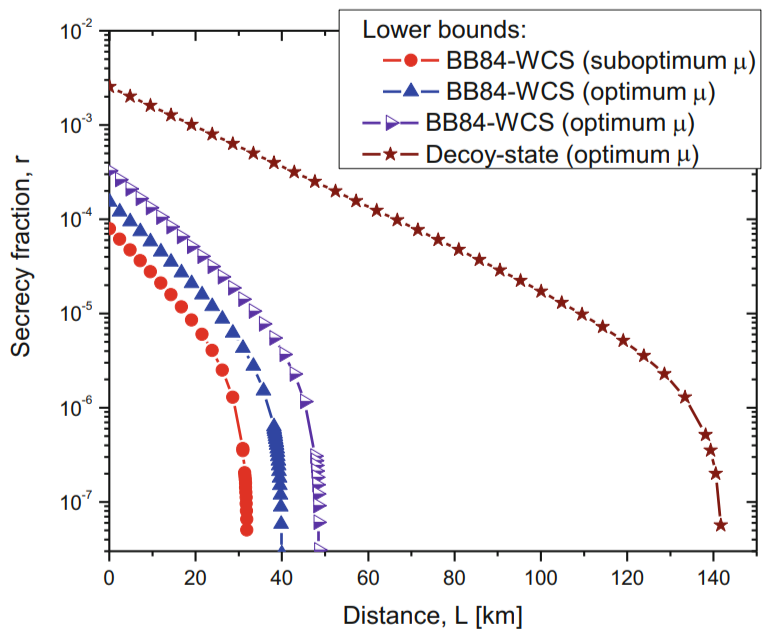
\includegraphics[width=0.8\textwidth]{chapters/figs/fig-8-1}
	\caption{کسر محرمانگی در مقابل مسافت ارسال برای پروتکل مبتنی بر حالت فریب و پروتکل \lr{BB84} مبتنی بر \lr{WCS}.}
	\label{fig:8-1}
\end{figure}






سایر پارامترهای استفاده شده در شبیه‌سازی‌ها به‌صورت زیر تنظیم شده‌اند \cite{8-10, 8-22, 8-23, 8-24}: بازدهی آشکارساز $\eta = 0.045$، نرخ شمارش تاریک $p_d = 1.7 \times 10^{-6}$، احتمال برخورد فوتون به آشکارساز اشتباه $e_d = 0.033$ و ناکارآمدی مصالحه $f_e = 1.22$. برای پروتکل \lr{BB84} مبتنی بر حالت فریب، جهت محاسبه کسر محرمانگی، از رابطه \eqref{eq:8-13} برای مقدار بهینه میانگین تعداد فوتون در هر پالس $\mu$ استفاده می‌کنیم؛ که در آن $q_\mu$ توسط $q_\mu = 1 - (1-y_0)\exp(-\mu T)$ تعیین می‌شود، $e_\mu$ توسط رابطه \eqref{eq:8-12}، $e_1$ توسط رابطه \eqref{eq:8-11} و $q_1$ به‌عنوان آرگومانِ \eqref{eq:8-1} برای $n=1$، یعنی توسط $q_1 = y_1 \mu \exp(-\mu)$ تعیین می‌گردد. برای پروتکل \lr{BB84} مبتنی بر \lr{WCS}، بدون حالت فریب، از رابطه \eqref{eq:8-4} با این فرض استفاده می‌کنیم که ایو کانال را کنترل کرده، حملات سد کردن-بازارسال را انجام می‌دهد و نسبت به حالت‌های چندفوتونی شفاف است. در این سناریوی کران پایین، خطا ناشی از رویدادهای تک‌فوتونی غالب است. اکنون با محاسبه $q^{(Z)}$ توسط $q_\mu = 1 - (1-y_0)\exp(-\mu T)$ و $e^{(Z)}$ توسط $E_\mu = e_d + (e_0 - e_d)y_0 / q_\mu$ و با فرض $\mu$ غیربهینه متناسب با $T$، منحنی قرمز در شکل \ref{fig:8-1} به‌دست آمد که با مرجع \cite{8-10} مطابقت دارد. هنگامی که به جای آن از $\mu$ بهینه (که کسر محرمانگی را بیشینه می‌کند) استفاده می‌کنیم، منحنی آبی به‌دست می‌آید که با مرجع \cite{8-23} مطابقت دارد. برای این دو منحنی، مقدار $q_1^{(Z)}$ را از \eqref{eq:7-6} با قرار دادن $y_n = 1$ برای $n \geq 2$ (ببینید مرجع \cite{8-22}) به‌صورت زیر تخمین می‌زنیم:
\begin{equation}
	q_1^{(X)} \geq q_\mu - \sum_{n=2}^{\infty} \frac{e^{-\mu} \mu^n}{n!}.
	\label{eq:8-14}
\end{equation}
با توجه به اینکه حالت‌های چندفوتونی خطایی ایجاد نمی‌کنند، یعنی برای $n \geq 2$ مقدار $e_n = 0$ است، می‌توانیم $e_1$ را به‌صورت زیر محدود کنیم:
\begin{equation}
	e_1^{(X)} \leq q_\mu E_\mu / q_1^{(X)}.
	\label{eq:8-15}
\end{equation}
رابطه دقیق‌تر برای $q_\mu$ در پروتکل \lr{BB84} مبتنی بر \lr{WCS}، به‌صورت زیر خواهد بود:
\begin{equation}
	q_\mu = y_0 e^{-\mu} + y_1 e^{-\mu} \mu + \sum_{n=2}^{\infty} \frac{e^{-\mu} \mu^n}{n!},
	\label{eq:8-16}
\end{equation}
که از \eqref{eq:7-6} با قرار دادن $y_n = 1$ برای $n \geq 2$ به‌دست می‌آید. منحنی متناظر با رنگ بنفش نشان داده شده است که نشان می‌دهد هنگام استفاده از پروتکل \lr{BB84} مبتنی بر \lr{WCS}، مسافت $L = 48.62$ کیلومتر دستیابی‌پذیر است. در مقابل، برای پروتکل \lr{BB84} مبتنی بر حالت فریب و $\mu$ بهینه، دستیابی به مسافت نزدیک به $141.8$ کیلومتر امکان‌پذیر است که با مرجع \cite{8-23} مطابقت دارد.






\section{امنیت سیستم‌های \lr{QKD} با منابع محدود}
\label{sec:8-2}

همان‌طور که در مرور کلی پروتکل \lr{BB84} بحث شد، پس از اتمام فاز ارسال کلید خام، آلیس و باب فرآیند غربال‌گری\LTRfootnote{Sifting procedure} و تخمین پارامتر\LTRfootnote{Parameter estimation} را انجام می‌دهند، به‌طوری که از $N$ نماد ارسال‌شده، $n$ نماد باقی می‌ماند و کلید متناظر با آن‌ها به‌عنوان کلید غربال‌شده\LTRfootnote{Sifted key} شناخته می‌شود. پس از آن، آن‌ها پس‌پردازش کلاسیک مانند مصالحه اطلاعات\LTRfootnote{Information reconciliation} و تقویت حریم خصوصی\LTRfootnote{Privacy amplification} را انجام می‌دهند. در مرحله مصالحه اطلاعات، آن‌ها از تصحیح خطا\LTRfootnote{Error correction} برای اصلاح خطاهای وارد شده توسط هر دو عاملِ کانال کوانتومی و ایو استفاده می‌کنند و کلید متناظر پس از اتمام این مرحله معمولاً کلید اصلاح‌شده\LTRfootnote{Corrected key} نامیده می‌شود. در طول تقویت حریم خصوصی، آن‌ها همبستگی باقی‌مانده با ایو را حذف می‌کنند و از $n$ نماد، $m$ نماد باقی می‌ماند که کلید متناظر، همان کلید امن\LTRfootnote{Secure key} است. به‌وضوح، نرخ کسریِ کلید مخفی $r$ را می‌توان به‌صورت $r = m/n$ (در حالت $N \to \infty$) تعیین کرد و اغلب از آن به‌عنوان کسر مخفی\LTRfootnote{Secret fraction} یاد می‌شود \cite{8-8}. نرخ کلید مخفی (\lr{SKR})\LTRfootnote{Secret-key rate (SKR)} سپس به‌صورت حاصل‌ضرب کسر مخفی و نرخ کلید خام، که با $R_{\text{raw}}$ نشان داده می‌شود، تعیین می‌گردد و می‌توانیم بنویسیم \cite{8-8}:
\begin{equation}
	\text{SKR} = r \cdot R_{\text{raw}}.
	\label{eq:8-17}
\end{equation}
\lr{QKD} می‌تواند به امنیت غیرمشروط\LTRfootnote{Unconditional security} دست یابد، به این معنی که امنیت آن را می‌توان بدون اعمال هیچ‌گونه محدودیتی بر توان محاسباتی یا استراتژی شنود ایو، تأیید کرد. کران‌های مربوط به نرخ کسر به مراحل پس‌پردازش کلاسیک بستگی دارند. رایج‌ترین روش، پس‌پردازش یک‌طرفه\LTRfootnote{One-way postprocessing} است که در آن آلیس یا باب کلید مرجع\LTRfootnote{Reference key} را در اختیار دارد و اطلاعات کلاسیک را از طریق کانال عمومی برای طرف دیگر ارسال می‌کند، در حالی که طرف مقابل بدون ارائه بازخورد، فرآیند خاصی را روی داده‌ها انجام می‌دهد. مشابه طرح‌های امنیت لایه فیزیکی\LTRfootnote{Physical-layer security (PLS)} (\lr{PLS}) توصیف شده در فصل \ref{chap:4}، معمول‌ترین پردازش یک‌طرفه شامل دو مرحله است: مصالحه اطلاعات و تقویت حریم خصوصی. عبارت کسر مخفی که از طریق پس‌پردازش یک‌طرفه به‌دست می‌آید، بسیار شبیه به طرح‌های \lr{PLS} کلاسیک است \cite{8-8}:
\begin{equation}
	r = I(\bm{A}; \bm{B}) - \min_{\text{\lr{Eve's strategies}}} (I_{EA}, I_{EB}),
	\label{eq:8-18}
\end{equation}
که در آن $I(\bm{A}; \bm{B})$ اطلاعات متقابل بین آلیس و باب است، در حالی که جمله دوم متناظر با اطلاعات ایو $I_E$ درباره کلید خام آلیس یا باب می‌باشد که در آن کمینه‌سازی روی تمام استراتژی‌های شنود ممکن انجام می‌شود. آلیس و باب تصمیم خواهند گرفت که از مصالحه مستقیم یا معکوس استفاده کنند تا بتوانند اطلاعات ایو را کمینه نمایند. در اینجا ما به امنیت در برابر حملات دسته‌جمعی\LTRfootnote{Collective attacks} علاقه‌مند هستیم. در بخش پیش‌ رو، توجه خود را به تعاریف مختلف امنیت معطوف می‌کنیم.





\subsection{نرخ کسر کلید مخفی با طول محدود}
\label{subsec:8-2-1}
فرض کنید کلید ایده‌آل\LTRfootnote{Perfect key} نشان‌دهنده دنباله‌ای از نمادهای کاملاً همبسته بین آلیس و باب باشد که ایو هیچ اطلاعاتی از آن‌ها در اختیار ندارد. کلید $K$ که به اندازه $\epsilon$ از کلید ایده‌آل انحراف داشته باشد، یک کلید $\epsilon$-امن\LTRfootnote{$\epsilon$-secure key} نامیده می‌شود. یکی از الزامات کلیدی که تعریف امنیت باید برآورده کند، ویژگی ترکیب‌پذیری\LTRfootnote{Composability property} است؛ بدین معنا که امنیت کلید صرف‌نظر از نوع کاربرد آن تضمین شده باشد \cite{8-8, 8-25, 8-26, 8-27, 8-28, 8-29}. به عبارت دیگر، اگر کلید $\epsilon$-امن در یک وظیفه $\epsilon'$-امن استفاده شود، کل فرآیند باید حداقل $(\epsilon + \epsilon')$-امن باشد.

\subsubsection{بازبینی $\epsilon$-امنیت مبتنی بر فاصله اثر}
\label{subsec:8-2-1-1}
برای مقابله با این مسئله، بن-اور\LTRfootnote{Ben-Or} و همکاران در \cite{8-25} و همچنین رنر\LTRfootnote{Renner} و کونیگ\LTRfootnote{König} در \cite{8-27} مفهوم $\epsilon$-امنیت مبتنی بر فاصله اثر\LTRfootnote{Trace-distance-based $\epsilon$-security} را معرفی کردند (همچنین ببینید \cite{8-28, 8-30, 8-31, 8-32, 8-33}). می‌گوییم کلید نسبت به شنودگر $E$ دارای $\epsilon$-امنیت است، اگر فاصله اثر بین حالت مشترک کلید $K$ و ایو $E$ (نشان داده شده با $\rho_{K,E}$) و حالت حاصل‌ضربِ حالت کاملاً مخلوط\LTRfootnote{Completely mixed state (CMS)} (\lr{CMS}) نسبت به مجموعه $K$ تمام کلیدهای امن ممکن (نشان داده شده با $\rho_{CMS}$) و حالت ایو (نشان داده شده با $\rho_E$)، کوچک‌تر یا مساوی $\epsilon$ باشد. به عبارت دیگر، می‌توانیم بنویسیم:
\begin{equation}
	D(\rho_{K,E}, \rho_{CMS} \otimes \rho_E) = \frac{1}{2} \|\rho_{K,E} - \rho_{CMS} \otimes \rho_E\|_1 = \frac{1}{2} \text{Tr} |\rho_{K,E} - \rho_{CMS} \otimes \rho_E| \leq \epsilon,
	\label{eq:8-19}
\end{equation}
که در آن $|\rho| = \sqrt{\rho^\dagger \rho}$ است. با این تعریف، پارامتر $\epsilon$ تفسیر کاملاً واضحی دارد؛ این پارامتر نشان‌دهنده حداکثر احتمال شکستِ تحمل‌پذیر برای فرآیند استخراج کلید است. با فرض برقرار بودن ویژگی ترکیب‌پذیری برای این تعریف، می‌توانیم امنیت کلید نهایی $\epsilon$ را برحسب امنیتِ گام‌های تصحیح خطا (\lr{EC})\LTRfootnote{Error correction (EC)} $\epsilon_{EC}$، تقویت حریم خصوصی (\lr{PA})\LTRfootnote{Privacy amplification (PA)} $\epsilon_{PA}$ و تخمین پارامتر (\lr{PE})\LTRfootnote{Parameter estimation (PE)} $\epsilon_{PE}$، و همچنین احتمال شکستِ تخمین‌های آنتروپی رنی\LTRfootnote{Rényi entropy} \cite{8-25} (نشان داده شده با $\epsilon_R$) تجزیه کنیم. به عبارت دیگر، می‌توانیم بنویسیم $\epsilon = \epsilon_{EC} + \epsilon_{PA} + \epsilon_{PE} + \epsilon_R$. کران‌های امنیتی بحث شده در بخش قبلی تنها به‌صورت مجانبی برای کلیدهای بی‌نهایت طولانی، زمانی که $\epsilon \to 0$ است، معتبر هستند. علاوه بر $\epsilon$-امنیت مبتنی بر فاصله اثر، می‌توان از مفهوم $\epsilon$-امنیت مبتنی بر وفاداری\LTRfootnote{Fidelity-based $\epsilon$-security} نیز استفاده کرد \cite{8-25}. با این حال، همان‌طور که در فصل \ref{chap:7} بحث شد، این دو رویکرد با یکدیگر معادل هستند.

اکنون پرسش اصلی این است که چگونه تعریف $\epsilon$-امنیت مبتنی بر فاصله اثر را به طول $m$ کلید مخفی استخراج‌شده مرتبط کنیم. برای این کار، نیاز است نامساوی زیر که نشان‌دهنده تعمیم کران چرنوف\LTRfootnote{Chernoff bound} است، اثبات شود \cite{8-8}:
\begin{equation}
	\text{Pr} \left( D(\rho_{K,E}, \rho_{CMS} \otimes \rho_E) > \epsilon \right) \leq e^{m - f(\rho_{K,E}, \epsilon)},
	\label{eq:8-20}
\end{equation}
که در آن از ضرایب ثابت صرف‌نظر شده است. به‌وضوح، کلید با احتمال بسیار کمی ناامن خواهد بود، به شرطی که شرط زیر برقرار باشد:
\begin{equation}
	m \leq f(\rho_{K,E}, \epsilon).
	\label{eq:8-21}
\end{equation}
به عبارت دیگر، تا زمانی که طول کلید کوتاه‌تر از عدم قطعیت ایو درباره ورودیِ مرحله تقویت حریم خصوصی باشد، کلید امن خواهد بود.

\subsubsection{کمینه-آنتروپی هموار و کسر کلید مخفی با طول محدود تحت حملات دسته‌جمعی}
\label{subsec:8-2-1-2}
آنتروپی رنی از مرتبه $\alpha$ برای متغیر $X$ می‌تواند به‌صورت زیر تعریف شود \cite{8-34}:
\begin{equation}
	R_\alpha(X) = \frac{1}{1 - \alpha} \log_2 \left( \sum_x [P_X(x)]^\alpha \right),
	\label{eq:8-22}
\end{equation}
که در آن $P_X(x)$ توزیع متغیر تصادفی $X$ است. کمینه-آنتروپی\LTRfootnote{Min-entropy} به‌عنوان حالت خاصی از آنتروپی رنی در حد $\alpha \to \infty$ تعریف می‌شود، یعنی:
\begin{equation}
	H_{\min}(X) = H_\infty(X) = \lim_{\alpha \to \infty} R_\alpha(X) = -\log_2 \max_{x \in \mathcal{X}} P_X(x).
	\label{eq:8-23}
\end{equation}
رنر در \cite{8-28} مفهوم کمینه-آنتروپی هموار\LTRfootnote{Smooth min-entropy} را برای پارامتر همواری $\epsilon > 0$ به‌صورت زیر معرفی کرد. فرض کنید $\mathcal{P}(\mathcal{H})$ نشان‌دهنده مجموعه عملگرهای غیرمنفی روی فضای هیلبرت\LTRfootnote{Hilbert space} $\mathcal{H}$ باشد. عملگر چگالی $\rho$ روی $\mathcal{H}$ غیرمنفی است اگر مزدوج هرمیتی با مقادیر ویژه غیرمنفی باشد. همچنین فرض کنید $\rho_{AB} \in \mathcal{P}(\mathcal{H}_A \otimes \mathcal{H}_B)$ و $\sigma_B \in \mathcal{P}(\mathcal{H}_B)$. کمینه-آنتروپی $\rho_{AB}$ نسبت به $\sigma_B$ طبق مرجع \cite{8-28} به‌صورت زیر تعریف می‌شود:
\begin{equation}
	H_{\min}(A|B) \doteq H_{\min}(\rho_{AB} | \sigma_B) = -\log \min \{ \lambda | \lambda \hat{I}_A \otimes \sigma_B - \rho_{AB} \geq 0 \},
	\label{eq:8-24}
\end{equation}
که در آن $\hat{I}_A$ عملگر همانی روی زیرفضای $A$ است. زمانی که $\mathcal{H}_B$ فضای بدیهیِ اعداد مختلط $\mathbb{C}$ باشد، کمینه-آنتروپیِ عملگر چگالی $\rho$ صرفاً به‌صورت زیر است:
\begin{equation}
	H_{\min}(\rho_A) = -\log \lambda_{\max}(\rho).
	\label{eq:8-25}
\end{equation}
کمینه-آنتروپی $\epsilon_R$-هموار برای $\rho_{AB}$ نسبت به $\sigma_B$ به‌صورت زیر تعریف می‌شود \cite{8-28}:
\begin{equation}
	H_{\min}^{\epsilon_R}(\rho_{AB} | \sigma_B) = \sup_{\bar{\rho}_{AB}} H_{\min}(\bar{\rho}_{AB} | \sigma_B),
	\label{eq:8-26}
\end{equation}
که در آن سوپریمم روی تمام عملگرهای $\bar{\rho}_{AB} \in \mathcal{P}(\mathcal{H}_A \otimes \mathcal{H}_B)$ گرفته می‌شود به‌طوری که $\text{Tr}(\bar{\rho}_{AB}) \leq \text{Tr}(\rho_{AB})$ و $\|\bar{\rho}_{AB} - \rho_{AB}\| \leq \epsilon_R \text{Tr}(\rho_{AB})$ باشد. اکنون پروتکل \lr{QKD}ای را در نظر بگیرید که در آن آلیس و باب $N$ جفت درهم‌تنیده را که با $\rho_{A^N B^N}$ نشان داده می‌شوند، به اشتراک می‌گذارند. آلیس و باب سپس اندازه‌گیری را روی کیوبیت‌های متناظر در جفت‌های درهم‌تنیده اعمال می‌کنند. برای اندازه‌گیری‌های فون نویمان\LTRfootnote{von Neumann measurements}، آلیس و باب مالک $N$ بیت با همبستگی بالا خواهند بود. در مرحله تخمین پارامتر، آلیس و باب زیرمجموعه‌ای شامل $p$ جفت همبسته را برای تعیین آمار $\lambda(A,B)$ داده‌های خود انتخاب می‌کنند. در فاز غربال‌گری برخی از جفت‌داده‌ها دور ریخته می‌شوند. برای آلیس و باب به‌ترتیب $n \leq N-p$ بیت باقی می‌ماند که نشان‌دهنده کلید خام است و با $X^n$ و $Y^n$ نشان داده می‌شوند. فرض کنید دنباله بیت‌هایی که ایو موفق به کسب آن‌ها شده است با $E^n$ نشان داده شود. در پس‌پردازش یک‌طرفه، آلیس و باب مراحل بیشتری از مصالحه اطلاعات (تصحیح خطا) و تقویت حریم خصوصی را انجام می‌دهند تا کلید امنی به طول $m \leq n$ به‌دست آورند. کمینه-آنتروپی هموار، تعداد بیت‌های یکنواختی را توصیف می‌کند که می‌توانند در مرحله تقویت حریم خصوصی استخراج شوند \cite{8-28, 8-29}. لم هش باقی‌مانده\LTRfootnote{Leftover hash lemma} از رمزنگاری کلاسیک \cite{8-35, 8-36} به ما می‌گوید که می‌توانیم $m < H_{\min}(X)$ بیت تقریباً به‌طور یکنواخت توزیع‌شده را با تقویت حریم خصوصی از یک متغیر تصارفی $X$ استخراج کنیم. به‌طور دقیق‌تر، برای تابع هشینگ جهانی-$2$ به‌صورت $h(S, X)$، که در آن $S$ روی مجموعه کلیدهای $\mathcal{S}$ یکنواخت است، اگر رابطه زیر برقرار باشد:
\begin{equation}
	m \leq H_{\min}(X) - 2\log \left( \frac{1}{\epsilon_{PA}} \right),
	\label{eq:8-27}
\end{equation}















آنگاه فاصله آماری\LTRfootnote{Statistical distance} محدود می‌شود به:
\begin{equation}
	\delta(h(S,X), (U,S)) \leq \epsilon_{PA},
	\label{eq:8-28}
\end{equation}
که در آن $U$ روی $\{0,1\}^m$ یکنواخت است. فاصله آماری برای دو متغیر تصادفی $\bm{Y}$ و $\bm{Z}$ به‌صورت زیر تعریف می‌شود:
\begin{equation}
	0 \leq \delta(\bm{Y}, \bm{Z}) = \frac{1}{2} \sum_v |Pr(\bm{Y} = v) - Pr(\bm{Z} = v)| \leq 1.
	\label{eq:8-29}
\end{equation}
نامساوی متناظر برای \lr{QKD} صرفاً تعمیمی از \eqref{eq:7-27} به‌صورت زیر خواهد بود:
\begin{equation}
	m \leq H_{\min}^{\epsilon_R}(\bm{X}^n | \bm{E}^n) - 2 \log \left( \frac{1}{\epsilon_{PA}} \right).
	\label{eq:8-30}
\end{equation}
برای استخراج دقیقِ \eqref{eq:8-30}، خواننده علاقه‌مند به مراجع \cite{8-28, 8-37} ارجاع داده می‌شود. فاصله متناظر معادل با \eqref{eq:8-29} به‌صورت زیر داده می‌شود:
\begin{equation}
	\Delta(A|B) = \min_{\sigma_B} \frac{1}{2} \|\rho_{AB} - \hat{I}_A \otimes \sigma_B\|_1, \quad \text{Tr}(\sigma_B) = \text{Tr}(\rho_B), \quad \sigma_B \in \mathcal{P}(\mathcal{H}_B).
	\label{eq:8-31}
\end{equation}
با بازآرایی نامساوی \eqref{eq:8-30}، به‌دست می‌آوریم:
\begin{equation}
	2^{m - H_{\min}^{\epsilon_R}(\bm{X}^n | \bm{E}^n)} \leq 2^{\log \epsilon_{PA}^2},
	\label{eq:8-32}
\end{equation}
که می‌تواند به‌صورت زیر ساده شود:
\begin{equation}
	\sqrt{2^{m - H_{\min}^{\epsilon_R}(\bm{X}^n | \bm{E}^n)}} \leq \epsilon_{PA}.
	\label{eq:8-33}
\end{equation}
اکنون با مقایسه \eqref{eq:8-33} و \eqref{eq:8-28}، نتیجه می‌گیریم که:
\begin{equation}
	\Delta(A|B) = \sqrt{2^{m - H_{\min}^{\epsilon_R}(\bm{X}^n | \bm{E}^n)}} \leq \epsilon_{PA}.
	\label{eq:8-34}
\end{equation}
برای در نظر گرفتن نشت اطلاعات ناشی از تصحیح خطا، باید نامساوی \eqref{eq:8-30} را به‌صورت زیر اصلاح کنیم:
\begin{equation}
	m \leq H_{\min}^{\epsilon_R}(\bm{X}^n | \bm{E}^n) - 2 \log \left( \frac{1}{\epsilon_{PA}} \right) - \text{leakage}_{EC}.
	\label{eq:8-35}
\end{equation}
در پروتکل‌های به کمک درهم‌تنیدگی\LTRfootnote{Entanglement assisted protocols}، آلیس و باب در ابتدا حالت چگالی را به‌صورت $\rho_{A^N B^N} = (\sigma_{AB})^{\otimes N}$ به اشتراک می‌گذارند که در آن $\sigma_{AB}$ یک حالت بل دو-کیوبیتی است. با توجه به اینکه پالایش‌های\LTRfootnote{Purification} مختلف انجام شده توسط ایو تحت تبدیل یکانی محلی\LTRfootnote{Local unitary transformation} معادل هستند، می‌توانیم بنویسیم $\rho_{X^N E^N} = (\sigma_{XE})^{\otimes N}$ به‌طوری که $\sigma_{XE} \in \Gamma$ باشد؛ که در آن $\Gamma$ مجموعه عملگرهای چگالی سازگار با آمار $\lambda(A,B)$ است، به‌جز برای احتمال $\epsilon'_R$. در مراجع \cite{8-28, 8-29, 8-30} نشان داده شده است که کمینه-آنتروپی هموار، برای $\epsilon_R > \epsilon'_R$، از پایین به‌صورت زیر محدود می‌شود:
\begin{equation}
	H_{\min}^{\epsilon_R}(\bm{X}^n | \bm{E}^n) \geq n \left( \min_{\sigma_{XE} \in \Gamma} S(\bm{X}|\bm{E}) - (2D + 3) \sqrt{\frac{\log(2/(\epsilon_R - \epsilon'_R))}{n}} \right),
	\label{eq:8-36}
\end{equation}
که در آن $D$ بعد سیستم و $S(\cdot|\cdot)$ نشان‌دهنده آنتروپی فون نویمان شرطی است.

عبارت متناظر برای کسر کلید مخفی با طول محدود تحت حملات دسته‌جمعی به‌صورت زیر در می‌آید:
\begin{equation}
	r_N = \frac{n}{N} \left[ \min_{\sigma_{XE} \in \Gamma} S(\bm{X}|\bm{E}) - S(\bm{X}|\bm{B}) - \frac{1}{n} \log \left( \frac{2}{\epsilon_{EC}} \right) - \frac{2}{n} \log \left( \frac{1}{\epsilon_{PA}} \right) - (2D + 3) \sqrt{\frac{\log(2/\epsilon_R)}{n}} \right].
	\label{eq:8-37}
\end{equation}
مجموعه حالت‌های $\Gamma$ این واقعیت را در نظر می‌گیرد که تخمین پارامتر\LTRfootnote{Parameter estimation} بر پایه $p$ نمونه استوار است. از قانون اعداد بزرگ\LTRfootnote{Law of large numbers} (قضیه ۱۲.۲.۱ در مرجع \cite{8-38}) می‌دانیم که برای نمونه‌های $X_1, \dots, X_p$ که مستقل و با توزیع یکسان (\lr{i.i.d.}) با توزیع $P(x)$ هستند، رابطه زیر برقرار است:
\begin{equation}
	\text{Pr} \left( \mathcal{D}(P_{x^n} \| P) > \epsilon_{PE} \right) \leq 2^{-p (\epsilon_{PE} - D \ln(p+1)/p)},
	\label{eq:8-38}
\end{equation}
که در آن $\mathcal{D}(\cdot \| \cdot)$ آنتروپی نسبی\LTRfootnote{Relative entropy} است. علاوه‌بر این، از لم ۱۲.۶.۱ در مرجع \cite{8-38} می‌دانیم که برای دو توزیع $P_1$ و $P_2$ رابطه زیر معتبر است:
\begin{equation}
	\mathcal{D}(P_1 \| P_2) \geq \frac{1}{2 \ln 2} \|P_1 - P_2\|_1^2.
	\label{eq:8-39}
\end{equation}
زمانی که آمار $\lambda_p$ با انجام اندازه‌گیری‌های \lr{POVM}\LTRfootnote{POVM measurements} با $D$ نتیجه روی $\sigma$ به‌دست آید، آنگاه برای هر $\epsilon_{PE} > 0$، حالت $\sigma$ در مجموعه زیر قرار خواهد گرفت \cite{8-28, 8-29}:
\begin{equation}
	\Gamma_\xi = \{ \sigma : \|\lambda_p - \lambda_\infty(\sigma)\| \leq \xi \}, \quad \xi = \sqrt{\frac{2 \ln(1/\epsilon_{PA}) + D \ln(p+1)}{p}},
	\label{eq:8-40}
\end{equation}
که در آن $\lambda_\infty(\sigma)$ توزیع احتمال مبتنی بر \lr{POVM} است.





\subsubsection{کسر کلید مخفی با طول محدود تحت حملات همدوس}
\label{subsec:8-2-1-3}
رابطه \eqref{eq:8-37} برای حملات دسته‌جمعی معتبر است، اما همان‌طور که در مرجع \cite{8-30} بحث شده است، می‌توان آن را به حملات همدوس\LTRfootnote{Coherent attacks} نیز تعمیم داد. فرض کنید $\epsilon_{\text{coh}}$ نشان‌دهنده حداکثر احتمال شکستِ تحمل‌پذیر تحت حملات همدوس باشد. با وارد کردن جایگذاری زیر \cite{8-30}:
\begin{equation}
	\epsilon = \epsilon_{\text{coh}} (N + 1)^{-(D^4 - 1)},
	\label{eq:8-41}
\end{equation}
نرخ کسر محرمانگی متناظر برای حملات همدوس به‌صورت زیر در می‌آید \cite{8-30}:
\begin{equation}
	r_{N,\text{coh}} = r_N - \frac{2(D^4 - 1) \log(N + 1)}{N}.
	\label{eq:8-42}
\end{equation}
رویکرد دیگر برای نرخ‌های مخفی با کلید محدود، به‌کارگیری قضیه بازنمایی دِ فینتی\LTRfootnote{de Finetti representation theorem} است \cite{8-28, 8-30, 8-39}. قضیه بازنمایی دِ فینتی، فاصله بین حالت $n$-قسمتی اصلی $\rho_{AB}$ و مخلوطی از حالت‌های حاصل‌ضرب\LTRfootnote{Mixture of product states} $\rho_{A^N B^N} = (\sigma_{AB})^{\otimes N}$ را محدود می‌کند؛ این حالت‌ها معمولاً زمانی به‌دست می‌آیند که حمله دسته‌جمعی توسط ایو اعمال شود \cite{8-28, 8-30, 8-39} و با نام حالت‌های فینتی-هیلبرت-اشمیت\LTRfootnote{Finetti-Hilbert-Schmidt states} شناخته می‌شوند. این قضیه زمانی که کسی بخواهد پروتکل‌های مختلف \lr{QKD} را در سطح حالت‌های کوانتومی مقایسه کند، بسیار دقیق (\textit{Tight}) است. با این حال، همان‌طور که در مرجع \cite{8-30} نشان داده شده است، نتایج نسبتاً بدبینانه‌ای برای نرخ‌های کلید مخفی با طول محدود ارائه می‌دهد. در مرجع \cite{8-40} نشان داده شده است که برای اهداف \lr{QKD} و برخی دیگر از کاربردهای پردازش اطلاعات کوانتومی، مطالعه فاصله بین دو نگاشت ناوردا نسبت به جایگشت\LTRfootnote{Permutation invariant maps} که پروتکل \lr{QKD} را پیاده‌سازی می‌کنند، کافی است. فرض کنیم $p$ بیت از $N_s < N$ بیت غربال‌شده برای تخمین پارامتر استفاده شوند و اثر جزئی $k$ سیستم گرفته شود تا برای ارضای شرایط قضیه دِ فینتی، به حالت حاصل‌ضرب نزدیک شویم. $n = N_s - p - k$ بیت باقی‌مانده نشان‌دهنده کلید خام هستند. فرض کنید $\rho_{| \theta \rangle^n}$ نشان‌دهنده خروجی ناوردا نسبت به دورانِ یک پروتکل \lr{QKD} باشد که به‌طور کلی (برای هر $| \theta \rangle$) به‌صورت حاصل‌ضرب نیست. این حالت را می‌توان در زیرفضای متقارن (ناوردا نسبت به جایگشت) از $\mathcal{H}^n$ به‌صورت $\rho_{| \theta \rangle^n} = \sum \pi | \theta \rangle^{\otimes (n-t)} \otimes | \phi \rangle^{\otimes t}$ نمایش داد، که در آن مجموع روی تمام جایگشت‌های ممکن $\pi$ است و $0 \leq t \leq p/2$ می‌باشد. پارامتر $t$ با فاصله بین $\rho_{| \theta \rangle^n}$ و حالت حاصل‌ضرب $n$-تایی خالص کامل مرتبط است و می‌تواند طبق مراجع \cite{8-28, 8-30} به‌صورت $t = (N_s/k)[2 \ln (2/\epsilon_{\text{deF}}) + D^4 \ln k]$ تعیین شود که در آن $\epsilon_{\text{deF}}$ خطای پارامتری‌کننده $t$ است. خطای کل برای حمله همدوس را اکنون می‌توان به‌صورت $\epsilon = \epsilon_{EC} + \epsilon_{PA} + \epsilon_R + \epsilon_{PE} + \epsilon_{\text{deF}}$ تجزیه کرد. حداکثر خطای تخمین پارامتر برای $p$ نمونه به‌صورت زیر در می‌آید \cite{8-30}:
\begin{equation}
	\xi(p) = \frac{1}{D - 1} \sqrt{\frac{2 \ln(1/\epsilon_{PA}) + D \ln(p + 1)}{p} + (1 + \ln 2) h_2(t/p)},
	\label{eq:8-43}
\end{equation}
که در آن پارامتر $k$ به‌صورت بهینه تعیین شده و $h_2(\cdot)$ تابع آنتروپی باینری است. عبارت متناظر برای نرخ کسر مخفی با طول محدود، برای قضیه دِ فینتی، تحت حملات همدوس به‌صورت زیر در می‌آید \cite{8-28, 8-30}:
\begin{equation}
	r_N = \frac{n}{N} \left[ \min_{\sigma_{XE} \in \Gamma} S(\bm{X}|\bm{E}) - S(\bm{X}|\bm{B}) - \frac{1}{n} \log \frac{2}{\epsilon_{EC}} - \frac{2}{n} \log \frac{1}{\epsilon_{PA}} - \frac{4}{n} (p+k) \log D - \frac{(\frac{5}{2}D + 4) \log(2/\epsilon_R)}{n} + h_2\left(\frac{t}{n}\right) \right].
	\label{eq:8-44}
\end{equation}
با این حال، همان‌طور که در مرجع \cite{8-30} نشان داده شده است، این نرخ کسر مخفی با طول محدود منجر به مقادیر بسیار بدبینانه‌ای برای \lr{SKR} می‌شود.

\subsection{تحلیل دقیق کلید محدود}
\label{sec:8-2-2}
نویسندگان در مرجع \cite{8-41} تعاریف امنیتی را برای در بر گرفتن هر دو مورد صحت\LTRfootnote{Correctness} کلید و $\epsilon$-محرمانگی\LTRfootnote{$\epsilon$-secrecy} (همان‌طور که توسط رنر معرفی شد \cite{8-28}) بسط دادند. پروتکل \lr{QKD} کلید $K$ را در سمت آلیس و کلید $K'$ را در سمت باب خروجی می‌دهد که هر دو دارای طول یکسانی، مثلاً $l$، هستند. می‌گوییم کلید \textit{صحیح} است اگر برای هر استراتژی که ایو اعمال می‌کند، آن‌ها همچنان به کلید یکسانی برسند، یعنی $K' = K$. می‌گوییم پروتکل \lr{QKD} دارای $\epsilon_c$-صحت است اگر $Pr[K' \neq K] \leq \epsilon_c$ باشد. از سوی دیگر، تعریف امنیت، تعمیمی از تعریف ارائه‌شده در رابطه \eqref{eq:8-19} است. می‌گوییم پروتکل $\epsilon_s$-محرمانه است اگر نسبت به پروتکل کاملاً محرمانه، $\epsilon_s$-تمایزناپذیر\LTRfootnote{$\epsilon_s$-indistinguishable} باشد. شرط $\epsilon_s$-محرمانگی را می‌توان به‌صورت زیر فرمول‌بندی کرد:
\begin{equation}
	\min_{\rho_E} (1 - p_{\text{abort}}) D(\rho_{K,E}, \rho_{CMS} \otimes \rho_E) = \frac{1 - p_{\text{abort}}}{2} \min_{\rho_E} \text{Tr} |\rho_{K,E} - \rho_{CMS} \otimes \rho_E| \leq \epsilon_s,
	\label{eq:8-45}
\end{equation}
که در آن $p_{\text{abort}}$ احتمال توقف\LTRfootnote{Abort} پروتکل است. پروتکلی که برای آن $0 = \epsilon_s$ باشد، در اینجا \textit{کاملاً محرمانه} نامیده می‌شود. می‌گوییم پروتکل \textit{امن} است اگر به‌طور هم‌زمان صحیح و محرمانه باشد. به بیان دقیق‌تر، می‌گوییم پروتکل $\epsilon$-امن است، اگر به‌طور هم‌زمان $\epsilon_c$-صحیح و $\epsilon_s$-محرمانه باشد، به‌طوری که $\epsilon_c + \epsilon_s \leq \epsilon$. در نهایت، می‌گوییم پروتکل \textit{صلب}\LTRfootnote{Robust} است اگر در غیاب ایو، با احتمال $\epsilon_r$ متوقف شود. به‌عنوان یک مثال توصیفی، یک پروتکل بدیهی که همیشه متوقف می‌شود امن است، اما منجر به هیچ کلید امنی نمی‌شود. پروتکل $\epsilon$-امن منجر به یک کلید امن به طول $l$ می‌شود. برای در نظر گرفتن صلبیت پروتکل، نرخ کسر محرمانگی با کلید محدود را به‌صورت زیر تعریف می‌کنیم \cite{8-41}:
\begin{equation}
	r = (1 - \epsilon_r) \frac{l}{N(n, p)},
	\label{eq:8-46}
\end{equation}
که در آن $N(n, p)$ نشان‌دهنده تعداد کیوبیت‌هایی است که باید ارسال شوند تا $n$ بیت کلید خام و $p$ بیت برای استفاده در تخمین پارامتر جمع‌آوری گردند. با استفاده از این مفهوم، برای منبع کوانتومی با کیفیت آماده‌سازی $q$، کلید $\epsilon$-امن است اگر نامساوی زیر برقرار باشد:
\begin{equation}
	l \leq n [1 - h_2(Q + \Delta Q)] - \text{leak}_{EC} - \log_2 \left( \frac{2}{\epsilon_s^2 \epsilon_c} \right), \quad \Delta Q = \sqrt{\frac{n + p}{np} \frac{p + 1}{p} \ln \left( \frac{2}{\epsilon_s} \right)},
	\label{eq:8-47}
\end{equation}
که در آن $Q$ حداکثر \lr{QBER} تحمل‌پذیر است و $\Delta Q$ متناظر با اصلاحی است که برای در نظر گرفتن نوسانات آماری اضافه می‌شود. بدیهی است که این تخمین دقیقِ طول کلید محدود برای پروتکل‌های دو‌بعدی قابل اعمال است. با این حال، می‌توان آن را مستقیماً به پروتکل‌های $D$-بعدیِ دو-پایه‌ای تعمیم داد. نشان داده شده است که نرخ‌های کسر محرمانگی متناظر برای $N$ به اندازه کافی بزرگ، با عبارات مبتنی بر تعریف رنر به‌خوبی مطابقت دارند، اما نتایج عددی نشان می‌دهند که نرخ‌های محرمانگی واقعی برای طول‌های کلید غربال‌شده‌ی $N$ کم و متوسط، بسیار بالاتر از مقادیر پیش‌بینی شده توسط تئوری رنر هستند.

\section{تحلیل کلید محدود برای پروتکل‌های QKD BB84 و حالت فریب روی کانال‌های تلاطم اتمسفری}
\label{sec:8-3}
در این بخش، تحلیل کلید محدود نرخ‌های کسر امن را برای پروتکل‌های \lr{BB84} مبتنی بر حالت همدوس ضعیف (\lr{WCS}) و حالت فریب در حضور اثرات تلاطم اتمسفری ارائه می‌دهیم \cite{8-21}. (توجه داشته باشید که در اینجا از نمادگذاری هماهنگ با این فصل استفاده می‌کنیم، نه نمادگذاری مرجع \cite{8-21}).





\subsection{پروتکل BB84 روی کانال‌های FSO متغیر با زمان}
\label{subsec:8-3-1}

تعداد فوتون‌های هر پالس سیگنال برای چنین منبع \lr{WCS}ای، از توزیع پواسون با پارامتر منبع $\mu$ پیروی می‌کند که نشان‌دهنده میانگین تعداد فوتون چشم‌داشتی\LTRfootnote{Expected average photon number} است. احتمال اینکه یک پالس همدوس ضعیف شامل $n$ فوتون باشد توسط $p_n = e^{-\mu} \mu^n / n!$ داده می‌شود و احتمال کل اینکه پالس‌ها شامل چندین فوتون باشند برابر است با $p_{\text{multi}} = \sum_{n \geq 2} p_n$. در چنین مواردی، گسیل گاه‌وبیگاهِ چندین فوتون از منبع، فرصتی را برای ایو فراهم می‌کند تا حمله تقسیم تعداد فوتون\LTRfootnote{Photon number splitting (PNS) attack} (\lr{PNS}) را انجام دهد (همچنین به فصل \ref{chap:7} مراجعه کنید). به‌منظور تضمین امنیت، شدت منبع (پارامتر $\mu$) با کاهش گذردهی کانال باید به‌طور اضافی تضعیف شود که این امر نرخ کسر امن دستیابی‌پذیر و حداکثر مسافت ارسال ممکن را به‌شدت کاهش می‌دهد. برای یک تلفات کانال معین، نرخ کسر امن به‌شدت به شدت منبع وابسته است. بر اساس نظریه کلید محدود محکم\LTRfootnote{Tight finite-key theory} \cite{8-41} که به‌اختصار در بخش قبلی شرح داده شد، نرخ کسر امن را به‌صورت زیر نمایش می‌دهیم \cite{8-21}:

\begin{equation}
	r = \frac{1}{2} p_{\exp} \left\{ \frac{p_{\exp} - p_{AE} p_{\text{multi}}}{p_{\exp}} [1 - h(Q + \Delta Q)] - \frac{\text{leak}_{EC}}{N} - \frac{1}{N} \log_2 \frac{2}{\epsilon_s^2 \epsilon_c} \right\},
	\label{eq:8-48}
\end{equation}

که در آن $Q$ همان \lr{QBER} است، در حالی که $\Delta Q \cong \sqrt{1/N \ln(1/\epsilon_s)}$ برای در نظر گرفتن نوسانات آماری ناشی از طول کلید محدود\LTRfootnote{Finite-size key length} معرفی شده است. احتمال آشکارسازی چشم‌داشتی توسط $p_{\exp} = 1 - \exp(-\mu T_B T)$ تعیین می‌شود که در آن $T_B$ نشان‌دهنده بازدهی کل آشکارسازی در سمت باب است و به‌عنوان حاصل‌ضرب گذردهی دهانه گیرنده $T_{Rx}$، گذردهی بخش نوری باب $\eta_B$، گذردهی آشکارساز $\eta_{\text{det}}$ و بازدهی کوانتومی آشکارساز\LTRfootnote{Quantum efficiency of detector} $\eta_{Qeff}$ تعیین می‌شود؛ یعنی $T_B = T_{RX} \eta_B \eta_{\text{det}} \eta_{Qeff}$. ما از $T = 10^{-\alpha L / 10}$ برای نشان دادن گذردهی کانال\LTRfootnote{Channel transmittance} استفاده می‌کنیم که در آن $\alpha$ ضریب تضعیف برحسب $\text{dB/km}$ و $L$ مسافت ارسال برحسب $\text{km}$ است. مطابق قبل، $h_2(\cdot)$ نشان‌دهنده تابع آنتروپی باینری است. علاوه‌بر این، \lr{QBER} را می‌توان به‌صورت $Q = Q_{\text{mis}} + 1/2 p_b$ تجزیه کرد که در آن $Q_{\text{mis}}$ احتمال وجود خطا در هر بازه زمانی به دلیل عدم‌انطباق\LTRfootnote{Misalignment} است و $p_b$ احتمال خطای نویز پس‌زمینه را نشان می‌دهد. احتمال خطای عدم‌انطباق توسط احتمالی که ایو حمله سد کردن-بازارسال\LTRfootnote{Intercept-resend (IR) attack} (\lr{IR}) را روی پالس‌های تک‌فوتونی انجام دهد ($p_{IR}$) تعیین می‌شود، به‌طوری که احتمال خطای عدم‌انطباق به‌صورت $Q_{\text{mis}} = 1/4 p_{IR} p_1 / p_{\exp}$ به‌دست می‌آید. نشت ناشی از تصحیح خطا توسط $\text{leak}_{EC} \approx f_{EC} h_2(Q)$ تخمین زده می‌شود که در آن $f_{EC}$ ناکارآمدی تصحیح خطا است و به‌صورت $f_{EC}(Q) \geq 1$ محدود می‌شود. پارامترهای امنیتی $\epsilon_c$ و $\epsilon_s$ به‌ترتیب نشان‌دهنده $\epsilon_c$-صحت\LTRfootnote{$\epsilon_c$-correctness} و $\epsilon_s$-محرمانگی\LTRfootnote{$\epsilon_s$-secrecy} هستند که در بخش قبلی تعریف شدند. $\epsilon$-امنیت کلِ پروتکل توسط $\epsilon \geq \epsilon_c + \epsilon_s$ تعیین می‌شود. در نهایت، $p_{AE}$ در رابطه \eqref{eq:8-48} نشان‌دهنده احتمال آشکارسازی در آشکارسازهای ایو است که به گذردهی بخش نوری آلیس $T_{\text{Alice}}$ و مکان ایو نیز بستگی دارد. موقعیت ایو بر انتخاب بهینه شدت منبع تأثیر خواهد گذاشت، همان‌طور که در ادامه نشان داده شده است. به‌صورت شهودی، هرچه ایو دسترسی بیشتری داشته باشد، نیاز بیشتری به تضعیف روشنایی منبع وجود دارد.

ما در غیاب تلاطم، شدت منبع بهینه $\mu$ را برای تلفات مختلف کانال و موقعیت‌های مختلف ایو محاسبه می‌کنیم که نتایج آن در شکل \ref{fig:8-2} خلاصه شده است.

\begin{figure}[ht]
	\centering
	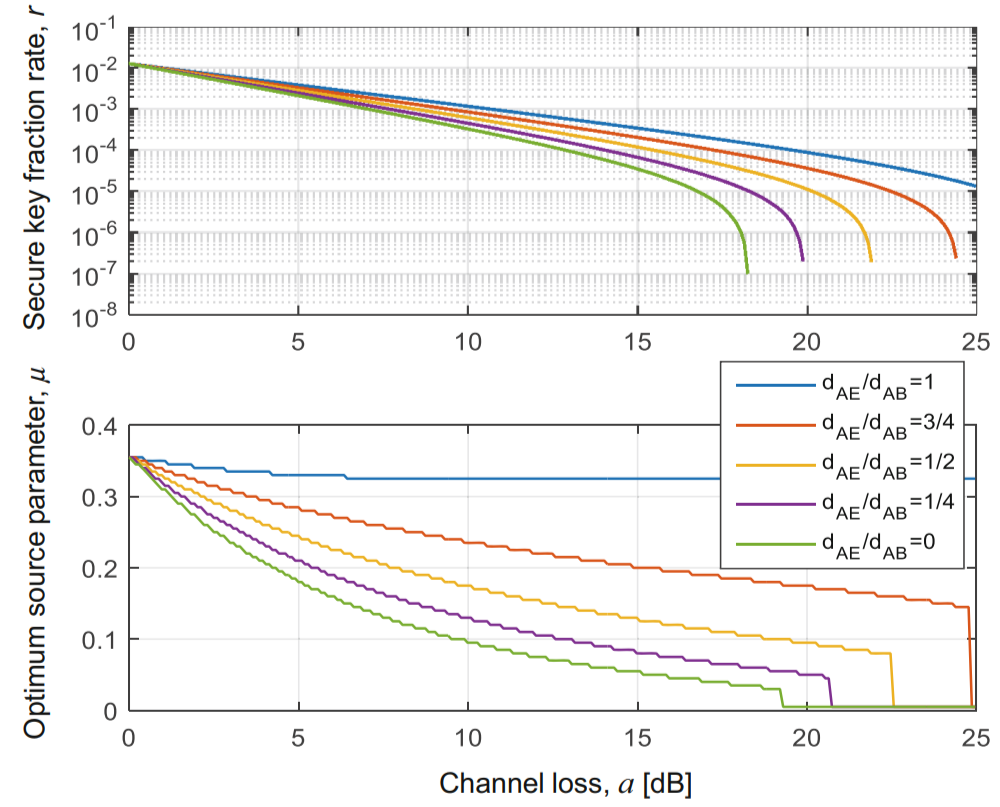
\includegraphics[width=\textwidth]{chapters/figs/fig-8-2}
	\caption{(بالا) نرخ کسر مخفی برحسب تلفات کانال به دسی‌بل، در حالی که ایو در فواصل مختلف از سمت باب ($d_{AE}/d_{AB} = 1$) تا سمت آلیس ($d_{AE}/d_{AB} = 0$) قرار دارد. (پایین) شدت منبع بهینه $\mu$ برحسب تلفات کانال (همچنین برحسب دسی‌بل). در محاسبات، پارامترها به‌صورت زیر انتخاب شده‌اند: $T_{\text{Alice}} = 0.4725$، $T_{Rx} = 0.7884$، $\eta_B = 0.898$، $\eta_{\text{det}} = 0.4352$، $\eta_{Qeff} = 0.9$، $\alpha = 0.192 \text{ dB/km}$، $p_b = 10^{-5}$، $f_{EC} = 1.16$، $N = 10^8$، $\epsilon_c = \epsilon_s = 10^{-6}$. (برگرفته از مرجع \cite{8-21}).}
	\label{fig:8-2}
\end{figure}

همان‌طور که از شکل پیداست، با افزایش تلفات کانال، هر دو مقدارِ نرخ کسر امن و پارامتر بهینه $\mu$ کاهش می‌یابند. با کاهش فاصله بین آلیس و ایو ($d_{AE}$)، که به معنای نزدیک‌تر شدن ایو به آلیس و کاهش نسبت $d_{AE}$ به کل فاصله $d_{AB}$ از ۱ (ایو در سمت باب) به ۰ (ایو در سمت آلیس) است، شدت منبع بهینه $\mu$ و در نتیجه نرخ کسر امن نیز کاهش می‌یابند.

اکنون مدل کانال متلاطم \lr{FSO} متغیر با زمان را شرح می‌دهیم \cite{8-21, 8-43}. باریکه نور هنگام انتشار در یک کانال \lr{FSO} متغیر با زمان، به دلیل توزیع تصادفی ضریب شکست، دچار اختلالات فاز و شدت می‌شود که با عنوان تلاطم\LTRfootnote{Turbulence} شناخته می‌شود \cite{8-43, 8-44, 8-45}. نوسان شدت یا تابش\LTRfootnote{Irradiance fluctuation} معمولاً به‌عنوان سنتیلاسیون\LTRfootnote{Scintillation} (چشمک‌زنی) شناخته می‌شود. اثر سنتیلاسیون در کانال‌های \lr{FSO} به‌طور گسترده مورد مطالعه قرار گرفته است تا تابع چگالی احتمال (\lr{PDF}) نوسانات تصادفی تابش استخراج شود. توزیع گاما-گاما ($\Gamma-\Gamma$) به‌عنوان مدل مناسبی برای سنتیلاسیون نوری در گستره رژیم‌های تلاطم ضعیف تا قوی عمل می‌کند که به‌صورت زیر داده می‌شود \cite{8-43, 8-44, 8-45}:

\begin{equation}
	p(I) = \frac{2 (\alpha\beta)^{(\alpha+\beta)/2}}{\Gamma(\alpha)\Gamma(\beta)} I^{(\alpha+\beta)/2 - 1} K_{\alpha-\beta} \left[ 2 (\alpha\beta I)^{1/2} \right], \quad I > 0,
	\label{eq:8-49}
\end{equation}

که در آن $I$ تابش نرمالیزه شده در گیرنده، $\Gamma(\cdot)$ تابع گاما و $K_p(\cdot)$ تابع بسل اصلاح‌شده\LTRfootnote{Modified Bessel function} نوع دوم و مرتبه $p$ است. پارامترهای $\alpha$ و $\beta$ به‌ترتیب نشان‌دهنده تعداد مؤثر سلول‌های مقیاس‌بزرگ و سلول‌های مقیاس‌کوچک در فرآیند پراکندگی هستند و به‌عنوان توابعی از واریانس ریتوف\LTRfootnote{Rytov variance} $\sigma^2_R$ تعریف می‌شوند که معمولاً به‌عنوان معیاری برای شدت تلاطم اتمسفری استفاده می‌شود. برای بررسی رابطه آن‌ها با واریانس ریتوف در حالت مقیاس درونی غیرصفر، خواننده علاقه‌مند به مرجع \cite{8-21} ارجاع داده می‌شود. تلاطم ضعیف با $\sigma^2_R < 1$، تلاطم متوسط با $\sigma^2_R \sim 1$ و رژیم تلاطم قوی با $\sigma^2_R > 1$ مشخص می‌شوند. رژیم موسوم به اشباع\LTRfootnote{Saturation regime} نیز با شرط $\sigma^2_R \to \infty$ تعیین می‌گردد.

برای مشخصه‌یابی فرکانسی سنتیلاسیون نوری، نوسانات شدت در بازه زمان همدوسی\LTRfootnote{Coherence time} اتمسفری به‌شدت همبسته هستند. زمان همدوسی که با $\tau_c$ نشان داده می‌شود، به‌عنوان حداقل مدت‌زمانی تعریف می‌شود که طی آن دو نمونه متوالی از شدت دریافتی ناهمبسته باشند. مطالعات بسیاری برای مدل‌سازی چگالی طیفی توان\LTRfootnote{Power spectral density (PSD)} (\lr{PSD}) سنتیلاسیون نوری برای هر دو مسیر افقی و عمودی انجام شده است، مانند \cite{8-46, 8-47}. مشخص شده است که طیف سنتیلاسیون مستقیماً با سرعت باد در طول کانال مرتبط است. فرمول‌های کلی در مرجع \cite{8-45} برای طیف‌های فرکانس زمانی سنتیلاسیون نوری برای هر دو نوع موج تخت و موج باریکه گاوسی ارائه شده است. \lr{PSD} برای محیط‌های مختلف از مکانی به مکان دیگر تغییر می‌کند و تحت تأثیر پارامترهای شرایط آب‌وهوایی مانند دما و رطوبت قرار می‌گیرد. یک مدل طیفی ساده از نوع باترورث\LTRfootnote{Butterworth-type} برای پیوندهای \lr{FSO} زمینی، که توسط دو پارامترِ فرکانس قطع و شیب طیفی تعیین می‌شود، در مرجع \cite{8-47} پیشنهاد شده است. این تابع انتقال توان به‌خوبی با شکل \lr{PSD} سنتیلاسیون نوری که از داده‌های تجربی برای یک پیوند افقی ۱ کیلومتری در یک محیط زمینی شهری استخراج شده است، مطابقت دارد \cite{8-47}. ما از این مدل باترورث مرتبه اول با فرکانس قطع $12$ هرتز در مدل کانال \lr{FSO} استفاده می‌کنیم تا به زمان همدوسی کانال در حدود $\tau_c \sim 10$ میلی‌ثانیه دست یابیم. برای به‌دست آوردن سنتیلاسیون نوری تحت تلاطم قوی، ابتدا دنباله‌ای از نمونه‌های تصادفی با توزیع نرمال ناهمبسته تولید کرده و سپس دنباله را توسط فیلتر باترورث فیلتر می‌کنیم. سپس هر نمونه را از توزیع نرمال به یک توزیع گاما-گاما (رابطه \eqref{eq:8-49}) با واریانس ریتوف $\sigma^2_R = 30$ با استفاده از تکنیک تبدیل غیرخطی بدون حافظه\LTRfootnote{Memoryless non-linear transform (MNLT)} (\lr{MNLT}) \cite{8-48} نگاشت می‌دهیم؛ این تکنیک با برابر قرار دادن توابع توزیع انباشته\LTRfootnote{Cumulative density functions (CDF)} (\lr{CDF}) آن‌ها، داده‌ها را از توزیع نرمال به توزیع گاما-گاما نگاشت می‌کند که در آن همبستگی موجود در دنباله حفظ می‌شود.








\lr{PSD}\LTRfootnote{Power Spectral Density} و \lr{PDF}\LTRfootnote{Probability Density Function} مدل کانال \lr{FSO} متغیر با زمان به‌ترتیب در شکل‌های \ref{fig:8-3} (\subref{fig:8-3-a} و \subref{fig:8-3-b}) نشان داده شده‌اند. زمان همدوسی\LTRfootnote{Coherence time} همان‌طور که هدف‌گذاری شده بود، تقریباً $10$ میلی‌ثانیه است. ما با فرض اینکه کانال در طول زمان همدوسی ثابت است (زیرا نمونه‌های شدت به‌شدت همبسته هستند)، مدل سنتیلاسیون\LTRfootnote{Scintillation} را به یک مدل محوشدگی بلوکی\LTRfootnote{Block fading} متغیر با زمان ساده می‌کنیم. همان‌طور که در شکل \ref{fig:8-3} (\subref{fig:8-3-b}) مشاهده می‌شود، \lr{PDF} مدل محوشدگی بلوکی به‌خوبی با توزیع تئوری گاما-گاما مطابقت دارد. ما همچنین فرض می‌کنیم که نوسانات در شدت دریافتی کاملاً ناشی از نوسانات در گذردهی کانال هستند؛ بنابراین بازدهی ارسال کانال، به‌عنوان مثال گذردهی کانال $\bm{T}$، با تابش دریافتی متناسب است که می‌تواند به‌عنوان حاصل‌ضرب گذردهی میانگین و توان دریافتی نرمالیزه‌شده‌ی حاصل از مدل محوشدگی بلوکی محاسبه شود.

\begin{figure}[ht]
	\centering
	\subfigure[]{\label{fig:8-3-a}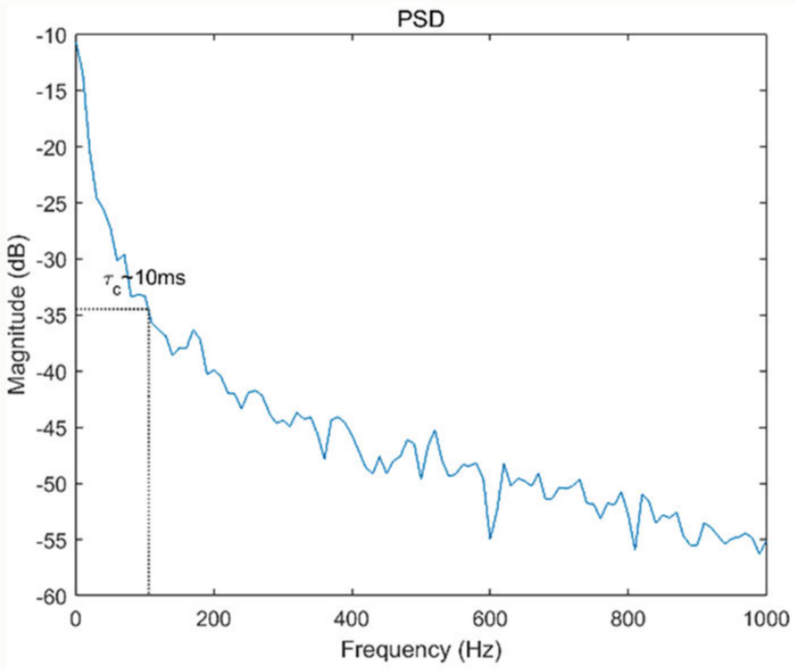
\includegraphics[width=0.48\textwidth]{chapters/figs/fig-8-3-a}}
	\hfill
	\subfigure[]{\label{fig:8-3-b}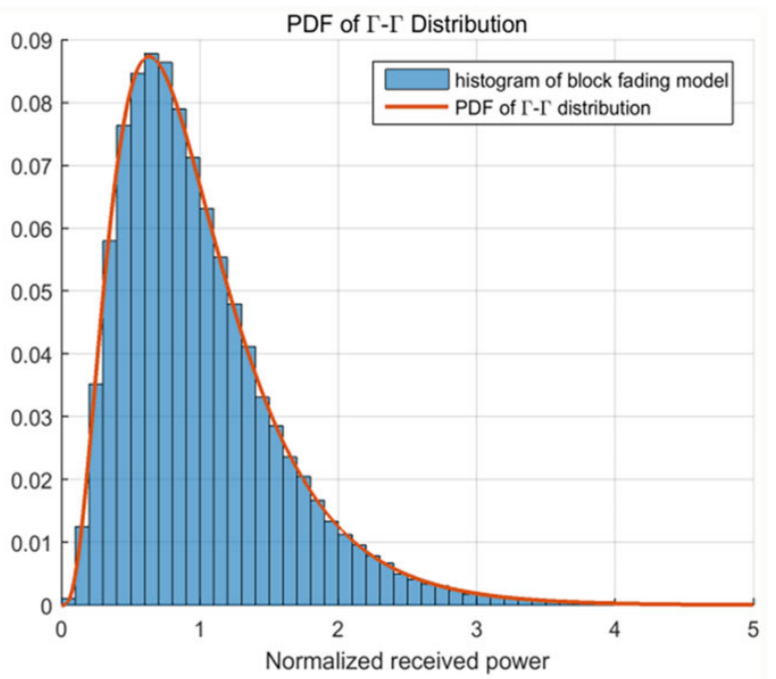
\includegraphics[width=0.48\textwidth]{chapters/figs/fig-8-3-b}}
	\caption{مدل کانال متغیر با زمان: (\subref{fig:8-3-a}) \lr{PSD} مدل محوشدگی بلوکی تولیدشده؛ (\subref{fig:8-3-b}) \lr{PDF} توزیع گاما-گاما با واریانس ریتوف $30$ و هیستوگرام مدل محوشدگی بلوکیِ تابش دریافتی نرمالیزه‌شده. (برگرفته از مرجع \cite{8-21}).}
	\label{fig:8-3}
\end{figure}

عملکرد نرخ‌های کسر امن در سیستم \lr{QKD} مبتنی بر \lr{FSO} می‌تواند به‌طور قابل‌توجهی تحت تأثیر اثرات تلاطم اتمسفری قرار گیرد. به‌طور معمول، اغلب بر اساس شرایط میانگین کانال، یک شدت منبع ثابت فرض می‌شد، در حالی که ماهیت متغیر با زمانِ کانال \lr{FSO} عموماً نادیده گرفته می‌شود. بنابراین، در حضور تلاطم، توان ارسال ثابت اغلب نسبت به گذردهی آنی کانال دارای عدم انطباق\LTRfootnote{Mismatch} بوده و در نتیجه منجر به کاهش امنیت می‌گردد.






برای مواجهه با شرایط متغیر زمانی کانال \lr{FSO}، ما یک روش تطبیقی را پیشنهاد دادیم که در آن کانال \lr{FSO} را با یک سیگنال کاوشگر کلاسیک کمکی پایش کرده، سپس حالات کانال را بر اساس حالات قبلی و فعلی پیش‌بینی می‌کنیم و درخشندگی منبع را مطابق با پیش‌بینی‌های کانال تطبیق می‌دهیم تا نرخ‌های کسر امن بهبود یابند \cite{8-21}. در یک سیستم \lr{FSO} واقع‌گرایانه، ممکن است تأخیری بین اندازه‌گیری حالت کانال و اعمال تنظیمات بر پارامترهای منبع وجود داشته باشد که می‌تواند ناشی از تأخیر انتشار فیزیکی در طول مسیر یا به دلیل برخی فرآیندهای پردازش سیگنال در سیستم باشد. در چنین حالتی، پیش‌بینی حالات کانال به‌صورت بی‌درنگ\LTRfootnote{Real-time} ضروری است. در روش تطبیقی ما، یک پیش‌بین خودواگرد\LTRfootnote{Autoregressive (AR) predictor} (\lr{AR}) در سمت آلیس برای پیش‌بینی اطلاعات وضعیت کانال استفاده می‌شود و دقت پیش‌بینی‌ها تعیین می‌کند که تا چه حد بهبود در این طرح تطبیقی حاصل می‌شود. یک مدل \lr{AR} را می‌توان به‌عنوان یک فیلتر با پاسخ ضربه نامحدود\LTRfootnote{Infinite impulse response (IIR)} (\lr{IIR}) در نظر گرفت و مسئله اصلی، تعیین ضرایب فیلتر به‌گونه‌ای است که میانگین مربعات خطا کمینه شود. طبق تعریف، یک مدل خودواگرد به‌صورت زیر داده می‌شود:
\begin{equation}
	y_t = \sum_{i=1}^{o} a_i y_{t-i} + \epsilon_t,
	\label{eq:8-50}
\end{equation}
که در آن $a_i$ ضرایب خودواگرد ($i = 1, \dots, o$)، متغیر $y_t$ نشان‌دهنده حالات متوالی کانال متغیر با زمان، $o$ مرتبه مدل و $\epsilon_t$ نشان‌دهنده خطای باقی‌مانده است که یک فرآیند نویز سفید با میانگین صفر فرض می‌شود. با استفاده از مدل \lr{AR} فوق، هر حالت کانال $y_t$ را می‌توان از روی $o$ حالت قبلی به‌صورت زیر پیش‌بینی کرد:
\begin{equation}
	\hat{y}_t = \sum_{i=1}^{o} a_i y_{t-i},
	\label{eq:8-51}
\end{equation}
که در آن $\hat{y}_t$ نشان‌دهنده تخمینی از حالت کانال $y_t$ است. خطای پیش‌بینی به‌صورت تفاضل بین حالت تخمینی و واقعی کانال تعریف می‌شود، یعنی $\epsilon_t = y_t - \hat{y}_t$. با افزایش مرتبه مدل \lr{AR}، عملکرد پیش‌بین بهبود می‌یابد. برای ارزیابی دقت روش \lr{AR}، معمولاً از ریشه میانگین مربعات خطا\LTRfootnote{Root mean square error (RMSE)} (\lr{RMSE}) بین مقادیر پیش‌بینی‌شده و واقعی حالات کانال استفاده می‌شود، همان‌طور که در شکل \ref{fig:8-4} تصویر شده است. ما یک پیش‌بین $AR(o)$ را بر اساس مدل محوشدگی بلوکی که پیش‌تر شرح داده شد مدل‌سازی کرده و پیش‌بینی تک‌گامه یا چندگامه را با مرتبه حداکثر $20$ انجام می‌دهیم. همان‌طور که در شکل \ref{fig:8-4} (\subref{fig:8-4-a}) نشان داده شده است، مقدار \lr{RMSE} در مرتبه $o = 3$ به‌سرعت افت کرده و سپس با افزایش مرتبه فیلتر به‌کندی کاهش می‌یابد. طول پیش‌بینی $K$ بر دقت پیش‌بینی تأثیر می‌گذارد که در شکل \ref{fig:8-4} (\subref{fig:8-4-b}) با عنوان پیش‌بینی «$K$-گام-جلوتر» نشان داده شده است. همان‌طور که انتظار می‌رفت، با افزایش طول پیش‌بینی، مقدار \lr{RMSE} افزایش می‌یابد.

\begin{figure}[ht]
	\centering
	\subfigure[]{\label{fig:8-4-a}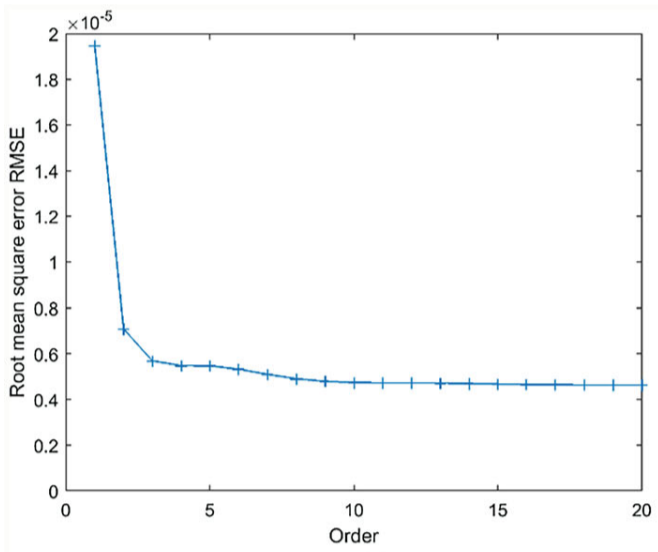
\includegraphics[width=0.45\textwidth]{chapters/figs/fig-8-4-a}}
	\hfill
	\subfigure[]{\label{fig:8-4-b}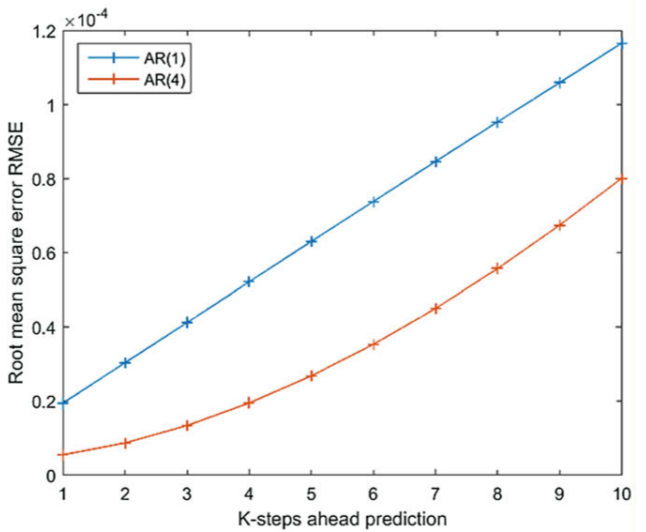
\includegraphics[width=0.45\textwidth]{chapters/figs/fig-8-4-b}}
	\caption{(\subref{fig:8-4-a}) ریشه میانگین مربعات خطا (\lr{RMSE}) برحسب مرتبه مدل \lr{AR}. (\subref{fig:8-4-b}) مقدار \lr{RMSE} برحسب طول پیش‌بینی $K$.}
	\label{fig:8-4}
\end{figure}

یک نمونه از بهبود حاصل از روش تطبیقی ما در شکل \ref{fig:8-5} تصویر شده است. در محاسبات، فرض کردیم که ایو در سمت آلیس قرار دارد ($d_{AE}/d_{AB} = 0$). منحنی آبی در وسط مربوط به نرخ کسر امن برای گذردهی میانگین کانال $T = T_{abs} T_{scatt}$ است که در آن گذردهی‌های جذب ($T_{abs}$) و پراکندگی ($T_{scatt}$) به‌ترتیب روی $0.9917$ و $0.365$ تنظیم شده‌اند. برای این مقدار میانگین، شدت منبع بهینه $\mu = 0.195$ برای بیشینه‌سازی نرخ کسر امن انتخاب شده است. زمانی که کانال \lr{FSO} در محوشدگی عمیق قرار دارد، همان‌طور که توسط منحنی زرد نشان داده شده است، باید درخشندگی منبع را برای تضمین امنیت کاهش دهیم. شدت بهینه به مقدار جدید $\mu = 0.135$ تغییر می‌کند. به‌سادگی از شکل دیده می‌شود که با کار در مقدار بهینه جدید، نرخ کسر امن از خط‌چین سیاه به خط‌چین خاکستری بهبود می‌یابد. مشابه بدترین حالت، زمانی که شرایط کانال بهتر می‌شود (مانند منحنی قرمز در بالا)، تطبیق شدت منبع با مقدار بهینه بالاترِ جدید $\mu = 0.25$ نیز باعث افزایش \lr{SKR} می‌گردد. به‌طور خلاصه، روش تطبیقی به منبع اجازه می‌دهد تا در درخشندگی بهینه (یا زیربهینه در صورتی که پیش‌بینی‌های وضعیت کانال خیلی دقیق نباشند) عمل کند.

\begin{figure}[ht]
	\centering
	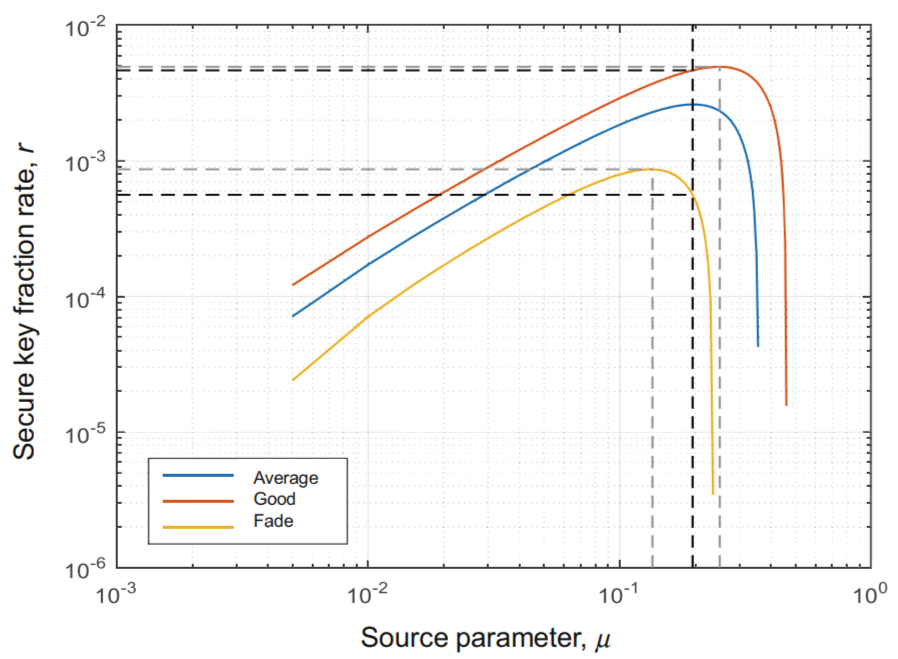
\includegraphics[width=0.8\textwidth]{chapters/figs/fig-8-5}
	\caption{تصویرسازی بهبود در نرخ کسر امن از طریق تطبیق درخشندگی منبع مبتنی بر مدل \lr{AR}. (برگرفته از مرجع \cite{8-21}).}
	\label{fig:8-5}
\end{figure}

با به‌کارگیری روش تطبیقی مبتنی بر مدل \lr{AR}، ما \lr{QKD} مبتنی بر \lr{BB84} را برای منبع همدوس ضعیف تحت رژیم تلاطم قوی با مدل‌سازی کانال \lr{FSO} متغیر با زمان به‌صورت مدل محوشدگی بلوکی شبیه‌سازی می‌کنیم. در اینجا از همان پارامترهای معرفی‌شده در بالا استفاده می‌کنیم. یک مدل ساده $AR(1)$ مرتبه اول، که توسط $1000$ نمونه اول در مدل کانال آموزش دیده است، برای پیش‌بینی حالات کانال در یک زمان همدوسی ($\tau_c$) و پنج زمان همدوسی جلوتر استفاده می‌شود. نرخ کسر امن با استفاده از رابطه \eqref{eq:8-48} برای هر زمان همدوسی محاسبه شده و سپس روی کل پالس‌های سیگنال ارسالی $N$ میانگین‌گیری می‌شود؛ نتایج عددی متناظر در شکل \ref{fig:8-6} خلاصه شده‌اند. روش تطبیق درخشندگی منبع در واقع نرخ کسر امن را در مقایسه با حالتی که از شدت منبع ثابت $\mu = 0.195$ (که برای شرایط میانگین کانال بهینه است) استفاده می‌شود، افزایش می‌دهد. برای منحنی «پیش‌بینی‌های کامل»، ما نرخ کسر امن را با این فرض تعیین می‌کنیم که حالات کانال به‌طور کامل پیش‌بینی شده‌اند. اگرچه چالش‌های فناورانه اساسی در ایجاد منابع تک‌فوتونی برحسب تقاضا همچنان امکان \lr{BB84} «خالص» را در نرخ داده‌های بالایی که در اینجا مد نظر ماست محدود می‌کند، اما هنگام مقایسه با نرخ کسر امنِ \lr{BB84} ایده‌آل با استفاده از منابع تک‌فوتونی، روش تطبیقی ما شکافِ ناشی از استفاده از منابع \lr{WCS} تجاری را کاهش می‌دهد. نسبت بهبود در نرخ کسر امن برای مورد جبران‌سازی کامل در پایین شکل \ref{fig:8-6} نشان داده شده است. علاوه‌بر این، عملکرد تطبیق درخشندگی منبع مبتنی بر روش \lr{AR} به دقت پیش‌بینی‌های حالت کانال بستگی دارد. با کاهش دقت پیش‌بینی هنگام افزایش طول پیش‌بینی، نرخ کسر امن در مقایسه با حالت ایده‌آل پیش‌بینی کامل کاهش می‌یابد. نرخ کسر امن متناظر با پیش‌بینی یک زمان همدوسی جلوتر، به‌طور نزدیکی به حالت پیش‌بینی کامل میل می‌کند.

\begin{figure}[ht]
	\centering
	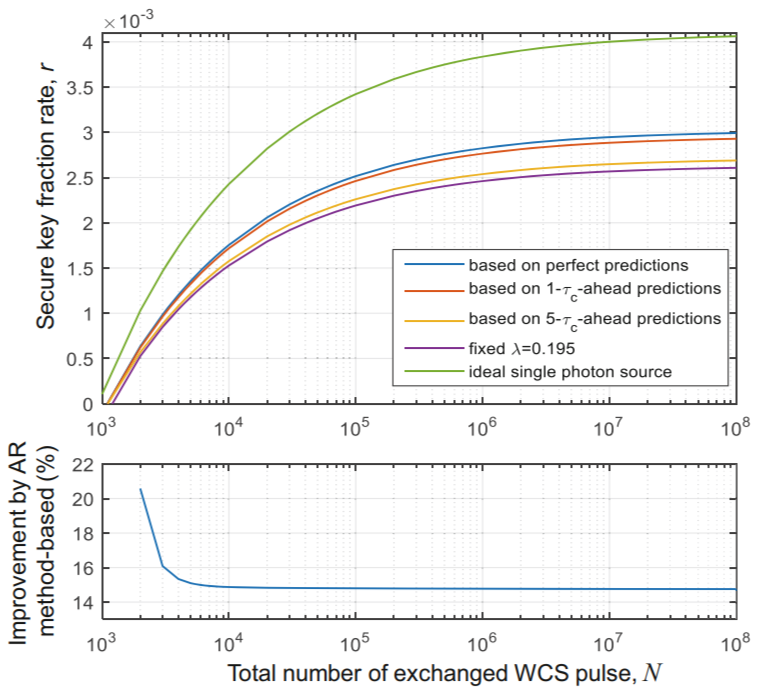
\includegraphics[width=0.8\textwidth]{chapters/figs/fig-8-6}
	\caption{بهبود در تطبیق مبتنی بر پیش‌بین \lr{AR}: (بالا) نرخ کسر امن برحسب تعداد کل پالس‌های \lr{WCS} مبادله‌شده ($N$)؛ (پایین) نسبت بهبود برای جبران‌سازی کامل برحسب $N$. (برگرفته از مرجع \cite{8-21}).}
	\label{fig:8-6}
\end{figure}

\subsubsection{پروتکل حالت فریب روی کانال‌های FSO متغیر با زمان}
\label{subsec:8-3-2}
برای بهینه‌سازی پروتکل مبتنی بر حالت فریب، ما از توصیف پروتکل ارائه شده در مرجع \cite{8-49} پیروی می‌کنیم. در این بخش، یک پروتکل حالت فریب مبتنی بر \lr{BB84} با سه حالت مختلف (یک حالت سیگنال و دو حالت فریب) مطالعه می‌شود. در مرجع \cite{8-50} نشان داده شده است که بهبود در نرخ کسر امن هنگام به‌کارگیری بیش از دو حالت فریب (علاوه بر حالت سیگنال) کمتر از $1\%$ است. در اینجا، ما از $\mu = \{\mu_1, \mu_2, \mu_3\}$ برای نشان دادن سه حالت مورد استفاده در پروتکل، و از $\lambda = \{\lambda_1, \lambda_2, \lambda_3\}$ برای نشان دادن شدت‌های منبع متناظر استفاده می‌کنیم. هر حالت با احتمال $p_{\mu_1} > p_{\mu_2} > p_{\mu_3} = 1 - p_{\mu_1} - p_{\mu_2}$ انتخاب می‌شود. با پیروی از تکنیک اثبات امنیت طول کلید محدود برای پروتکل مبتنی بر حالت‌های فریب بر اساس رابطه عدم قطعیت برای آنتروپی‌های هموار \cite{8-28, 8-29, 8-41, 8-51}، نرخ کسر کلید امن برای یک پروتکل حالت فریب با پایه‌های بدون سوگیری، که در آن دو پایه متقابل به‌طور یکسان انتخاب می‌شوند، به‌صورت زیر داده می‌شود:
\begin{equation}
	r \leq \frac{1}{2} \left[ \underline{Q}^{(0)} + \underline{Q}^{(1)} - \overline{Q}^{(1)} h(\bar{e}^{(1)}) - \frac{\text{leak}_{EC}}{N} - \Delta(N) \right],
	\label{eq:8-52}
\end{equation}
که در آن کران پایین و کران بالا به‌ترتیب با خط زیرین و خط بالایی نشان داده شده‌اند. در رابطه \eqref{eq:8-52}، $Q^{(n)}$ نشان‌دهنده نرخ آشکارسازی در سمت باب است که ناشی از سیگنال‌های با $n$ فوتون گسیل‌شده از منبع آلیس می‌باشد. با $e$ نرخ کل \lr{QBER} و با $e^{(n)}$ نرخ \lr{QBER} برای پالس‌های $n$-فوتونی را نشان داده‌ایم. مشابه قبل، $h_2(x)$ نشان‌دهنده تابع آنتروپی باینری است. پارامتر $\text{leak}_{EC}$ متناظر با نشت اطلاعات ناشی از تصحیح خطا (مصالحه اطلاعات) است. این بخش از اطلاعات باید هنگام محاسبه نرخ کسر امن کسر شود، زیرا ایو می‌تواند این بیت‌ها را صرفاً با انشعاب گرفتن از کانال کلاسیک تعیین کند. معمولاً این مقدار به‌صورت $\text{leak}_{EC} \approx Q f_{EC} h(e)$ تقریب زده می‌شود که در آن $Q$ نرخ کل آشکارسازی و $f_{EC}$ ناکارآمدی تصحیح خطا است. آخرین جمله در رابطه \eqref{eq:8-52} یعنی $\Delta(N)$، مربوط به امنیت تحت اثر اندازه محدود است که به‌صورت زیر تخمین زده می‌شود:
\begin{equation}
	\Delta(N) = \frac{1}{N} \log_2 \left( \frac{2}{\epsilon_c} \right) + \frac{6}{N} \log_2 \left( \frac{46}{\epsilon_s} \right).
	\label{eq:8-53}
\end{equation}
مشابه بخش قبلی، پروتکل \lr{QKD} مبتنی بر حالت‌های فریب زمانی $\epsilon$-امن (یا به‌طور دقیق‌تر $\epsilon_c$-صحیح و $\epsilon_s$-محرمانه) نامیده می‌شود که $\epsilon \geq \epsilon_s + \epsilon_c$ باشد. کران‌های پایین و بالا در رابطه \eqref{eq:8-52} با استفاده از نامساوی هوفدینگ\LTRfootnote{Hoeffding’s inequality} \cite{8-52} و بهینه‌سازی مقید تعیین می‌شوند. به‌طور مشخص‌تر، مقادیر قابل اندازه‌گیری در پروتکل، مانند تعداد آشکارسازی‌ها و تعداد خطاها، توسط نامساوی هوفدینگ از مقادیر مجانبی محدود می‌شوند: $x_{asym} - x \leq \sqrt{(x/2) \ln(1/\epsilon)}$ با احتمال شکست $2\epsilon$. سپس این کران‌ها به‌عنوان محدودیت‌های مسئله بهینه‌سازی برای تخمین مقادیری که مستقیماً قابل اندازه‌گیری نیستند، استفاده می‌شوند. برای مثال، از برنامه‌ریزی خطی برای به‌دست آوردن نرخ آشکارسازی سیگنال‌های $n$-فوتونی $\underline{q}_{\mu_i}^{(n)}$، که از پالس‌های آماده‌شده توسط آلیس در حالت $\mu_i$ ناشی می‌شوند، استفاده می‌شود:
\begin{equation}
	\min \underline{q}_{\mu_i}^{(n)},
	\label{eq:8-54}
\end{equation}
تحت قیود:
\begin{equation}
	\begin{aligned}
		\underline{Q}_{\mu_i} \leq \sum_{n=0}^{\infty} q_{\mu_i}^{(n)} e^{-\lambda_i} \frac{\lambda_i^n}{n!} \leq \overline{Q}_{\mu_i}, \quad n \in \{0, 1\}, \quad i \in \{1, 2, 3\} \\
		0 \leq q_{\mu_i}^{(n)} \leq 1, \quad n \in \{0, 1\}, \quad i \in \{1, 2, 3\}
	\end{aligned}
	\label{eq:8-55}
\end{equation}
که در آن $Q_{\mu_i} = C_{\mu_i} / N_{\mu_i}$ نرخ آشکارسازی برای هر حالت $\mu_i$ است، و $C_{\mu_i}$ و $N_{\mu_i}$ به‌ترتیب تعداد کل سیگنال‌هایی هستند که در حالت $\mu_i$ آشکار و ارسال شده‌اند. سپس کران‌های نرخ آشکارسازی پالس‌های $n$-فوتونی به‌صورت $\underline{Q}^{(n)} = \left[ \frac{N_{\mu_i}}{N} \underline{q}_{\mu_i}^{(n)} e^{-\lambda_i} \frac{\lambda_i^n}{n!} \right]$ داده می‌شود. مسئله بهینه‌سازی برای کران بالای \lr{QBER} تک‌فوتونی $\bar{e}^{(1)}$ را می‌توان با رابطه زیر ساده کرد \cite{8-53}:
\begin{equation}
	\bar{e}^{(1)} \leq \frac{e^{\lambda_i} e_{\mu_i} - \frac{1}{2} \underline{q}_{\mu_i}^{(0)}}{\lambda_i \underline{q}_{\mu_i}^{(1)}},
	\label{eq:8-56}
\end{equation}
که در آن $e_{\mu_i} = E_{\mu_i} / N_{\mu_i}$ نرخ \lr{QBER} از هر حالت $\mu_i$ است و $E_{\mu_i}$ تعداد کل خطاهایی است که در حالت $\mu_i$ آشکار شده‌اند. بهینه‌سازی عددی برای تعیین پارامترهای بهینه پروتکل حالت‌های فریب انجام شده است که نتایج عددی آن در شکل \ref{fig:8-7} برای تعداد کل پالس‌های سیگنال مبادله‌شده $N = 10^8$ خلاصه شده است. به‌وضوح، شدت منبع برای حالت سیگنال نیازی به کاهش خطی با گذردهی کانال ندارد و مقدار بهینه در سطح نسبتاً بالای $\lambda \sim 1$ باقی می‌ماند. با افزایش تلفات کانال، به دلیل پایین بودن نرخ آشکارسازی، حالت‌های فریب قوی‌تر برای تخمین آمار تک‌فوتونی بیشتر مورد نیاز هستند. توجه داشته باشید که نتایج عددی ما نشان می‌دهند که یکی از حالت‌های فریب همیشه در شدت صفر بهینه است، که با تحلیل مرجع \cite{8-54} که چنین حالتی را «حالت فریب خلاء» می‌نامد، مطابقت دارد.
%
\begin{figure}[ht]
	\centering
	\subfigure[]{\label{fig:8-7-a}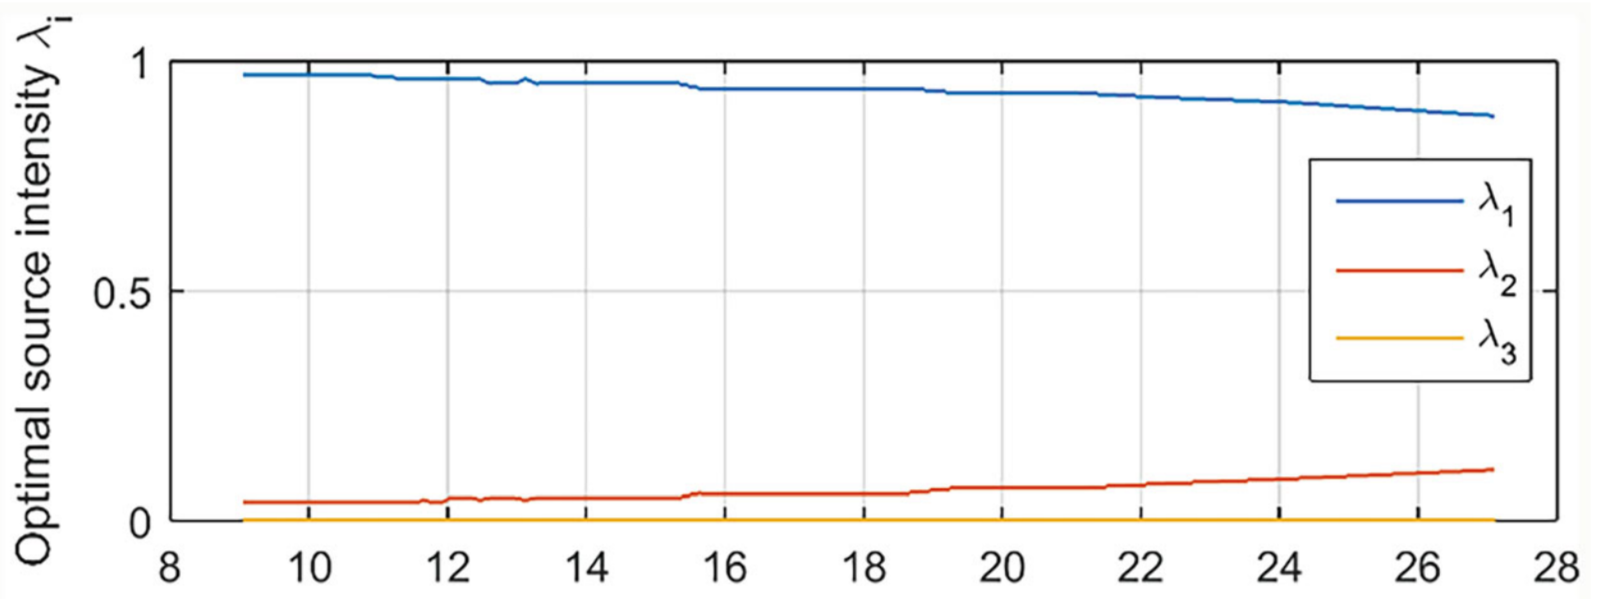
\includegraphics[width=.8\textwidth]{chapters/figs/fig-8-7-a}}
	
	
	\subfigure[]{\label{fig:8-7-b}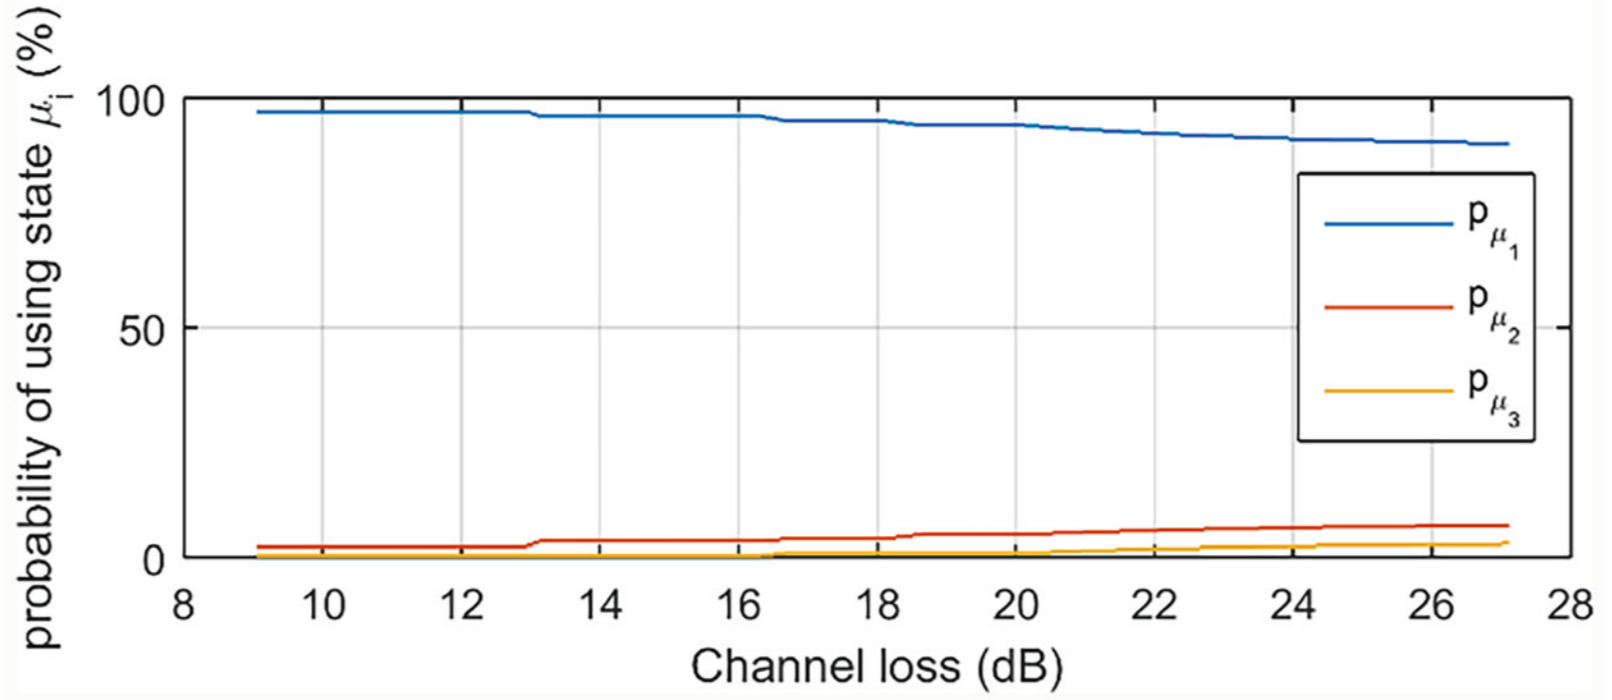
\includegraphics[width=0.8\textwidth]{chapters/figs/fig-8-7-b}}
	\caption{پارامترهای بهینه پروتکل دو-حالت-فریب در مقابل تلفات آنی کانال ناشی از تلاطم: (\subref{fig:8-7-a}) شدت منبع بهینه برحسب تلفات کانال به دسی‌بل؛ (\subref{fig:8-7-b}) احتمال ($\%$) استفاده آلیس از هر حالت برحسب تلفات کانال. (برگرفته از مرجع \cite{8-21}).}
	\label{fig:8-7}
\end{figure}

مشابه \lr{BB84} مبتنی بر \lr{WCS}، \lr{QKD} حالت فریب مبتنی بر \lr{FSO} نیز تحت تأثیر اثرات تلاطم اتمسفری قرار می‌گیرد. ما پروتکل حالت فریب شرح داده شده در بالا را تحت تلاطم قوی با تطبیق مبتنی بر پیش‌بین \lr{AR} شبیه‌سازی می‌کنیم. همان مقادیر امنیتی $\epsilon_c = \epsilon_s = 10^{-6}$ و نویز پس‌زمینه $p_b = 10^{-5}$ که در پروتکل \lr{BB84} مبتنی بر \lr{WCS} استفاده شده بود، در اینجا نیز به کار گرفته شده است. همان‌طور که در شکل \ref{fig:8-8} نشان داده شده است، نرخ‌های کسر امن با روش تطبیقی مبتنی بر پیش‌بین \lr{AR} بهبود می‌یابند و سطح بهبود عملکرد نرخ کسر کلید امن به دقت پیش‌بینی‌ها بستگی دارد. نرخ‌های کسر امن از بالا توسط حالت پیش‌بینی کامل محدود می‌شوند. در مقایسه با پروتکل‌های \lr{BB84}، از آنجا که نرخ کسر امن در پروتکل حالت فریب به‌صورت خطی با گذردهی کانال مقیاس‌بندی می‌شود \cite{8-55}، بهبود حاصل از تطبیق شدت منبع کمتر است. برای حالت پارامتر ثابت، پارامترهای بهینه تحت فرض مجانبی محاسبه شده‌اند؛ بنابراین همان‌طور که انتظار می‌رود، زمانی که تعداد کل پالس‌های سیگنال ارسالی $N$ بزرگ باشد، عملکرد بهتری دارد. بهبود تطبیقی برحسب نرخ کسر امن نسبت به تطبیق کامل، از $20\%$ در $N = 10^6$ به $5\%$ در $N = 10^9$ کاهش می‌یابد. مورد پیش‌بینی یک زمان همدوسی جلوتر، به‌طور نزدیکی به مورد تخمین کامل کانال میل می‌کند و برای تمام مقادیر $N$ مفید است. با این حال، دقت پیش‌بینی‌های پنج زمان همدوسی جلوتر برای تمام مقادیر $N$ در مقایسه با \lr{BB84} به اندازه کافی خوب نیست. زمانی که $N$ بزرگ است، جایی که مورد پارامتر ثابت به‌خوبی عمل می‌کند، روش تطبیقی به دلیل عدم‌انطباق ناشی از پیش‌بینی‌های ضعیف حالت کانال، منجر به نرخ کلید کسر امن پایین‌تری می‌شود. از این منظر، پروتکل حالت فریب به دقت پیش‌بینی بالاتری نسبت به \lr{BB84} اصلی نیاز دارد. به عبارت دیگر، پروتکل مبتنی بر حالت فریب در مقایسه با پروتکل \lr{BB84} نسبت به اثرات تلاطم اتمسفری صلب‌تر است، به‌طوری که تطبیق مبتنی بر پیش‌بین \lr{AR} در این مورد برای $N$ به اندازه کافی طولانی کمک چندانی نمی‌کند.

\begin{figure}[ht]
	\centering
	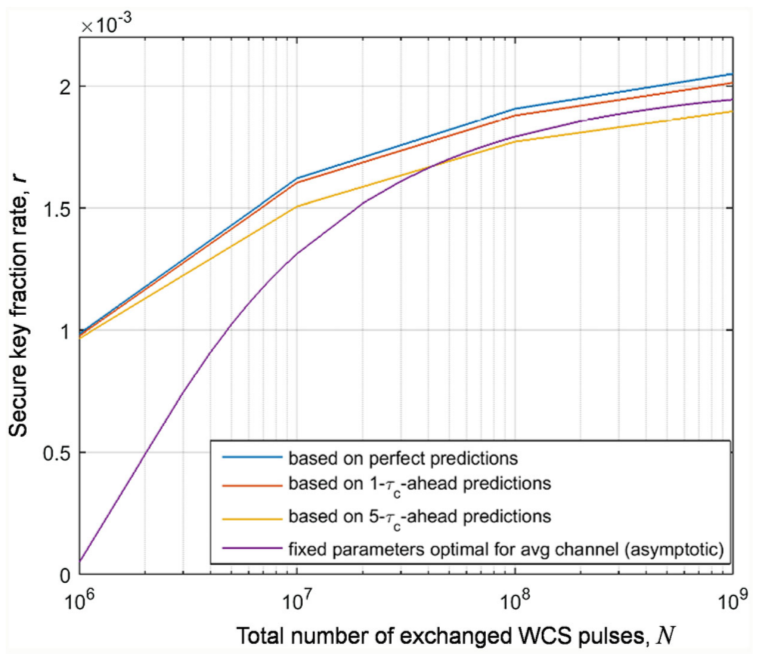
\includegraphics[width=0.8\textwidth]{chapters/figs/fig-8-8}
	\caption{نرخ کسر کلید امن برحسب تعداد کل پالس‌های سیگنال ارسالی ($N$) برای \lr{QKD} مبتنی بر حالت فریب با تطبیق مبتنی بر روش \lr{AR}. (برگرفته از مرجع \cite{8-21}).}
	\label{fig:8-8}
\end{figure}

\section{پروتکل‌های DV-QKD با ابعاد بالا}
\label{sec:8-4}
به‌رغم ویژگی‌های جذاب \lr{QKD}، دو چالش بنیادی و فنی وجود دارد که باید پیش از کاربردهای گسترده آن مورد توجه قرار گیرند. نخست، نرخ کلید مخفی \lr{QKD} به‌طور بنیادی توسط تلفات کانال محدود می‌شود، که توسط مصالحه نرخ-تلفات\LTRfootnote{Rate-loss tradeoff} کمی‌سازی می‌گردد \cite{8-56, 8-57, 8-58}. تکرارکننده‌های کوانتومی\LTRfootnote{Quantum repeaters} راه حل نهایی برای غلبه بر تلفات کانال خواهند بود، اما در حال حاضر فراتر از دسترس فناوری‌های موجود هستند. یک راه حل نزدیک‌مدت، کدگذاری اطلاعات کوانتومی در یک فضای هیلبرت با بعدی بالاتر از کدگذاری دو‌بعدیِ رایج (مانند استفاده از حالات قطبش فوتون‌ها) است. یک فضای کدگذاری با ابعاد بالا\LTRfootnote{High-dimensional (HD) encoding} تضمین می‌کند که با دریافت هر تک‌فوتون، چندین بیت اطلاعات تحویل داده شود؛ بدین ترتیب بازدهی فوتون برای \lr{QKD} با نرخ بالا در غیاب تکرارکننده‌های کوانتومی بهینه می‌شود \cite{8-59}. چندین رویکرد اخیراً برای افزایش بعد فضای کدگذاری تک‌فوتون‌ها دنبال شده است. این رویکردها یا از پارامترهای ابعاد بالا مانند بازه زمانی\LTRfootnote{Time bin}، کیوبیت‌های فرکانسی \cite{8-60, 8-61}، مکان و تکانه خطی \cite{8-62, 8-63, 8-64}، تکانه زاویه‌ای مداری (\lr{OAM}) \cite{8-32, 8-33, 8-65, 8-66, 8-67, 8-68, 8-69, 8-70, 8-71, 8-72} بهره می‌برند، و یا به‌طور هم‌زمان از چندین پارامتر کدگذاری‌شده در حالت‌های فوق-درهم‌تنیده\LTRfootnote{Hyper-entangled states} استفاده می‌کنند \cite{8-73, 8-74}. علاوه‌بر این، اخیراً پیشنهاد شده است که از توری‌های براگ فیبری (\lr{FBG}) با پاسخ ضربه متعامد متقابل به‌عنوان پایه کدگذاری برای \lr{HD-QKD} استفاده شود \cite{8-31}. متناوباً، همان‌طور که در \cite{8-75} پیشنهاد شده است، \lr{FBG}ها می‌توانند با توری‌های براگ موجبری (\lr{WBG}) که به‌صورت الکترونیکی قابل کنترل هستند، جایگزین شوند. پیش از ادامه بحث درباره سیستم‌های \lr{HD-QKD}، جزئیات بیشتری درباره پایه‌های متقابلاً بدون سوگیری (\lr{MUB}) برای سیستم‌های ابعاد بالا ارائه می‌دهیم \cite{8-31, 8-76, 8-77, 8-78, 8-79}.







\subsection{پایه‌های متقابلاً بدون سوگیری (\lr{MUBs})}
\label{subsec:8-4-1}
دو پایه متعامد\LTRfootnote{Orthonormal bases} $\{|e_1\rangle, \dots, |e_D\rangle\}$ و $\{|f_1\rangle, \dots, |f_D\rangle\}$ در فضای هیلبرت\LTRfootnote{Hilbert space} $\mathbb{C}^D$ زمانی پایه‌های متقابلاً بدون سوگیری\LTRfootnote{Mutually Unbiased Bases (MUBs)} (\lr{MUB}) هستند که مجذور اندازه ضرب داخلی\LTRfootnote{Inner product} بین هر دو حالت پایه $\{|e_m\rangle\}$ و $\{|f_n\rangle\}$ برابر با معکوس بُعد باشد:
\begin{equation}
	|\langle e_m | f_n \rangle|^2 = \frac{1}{D} \quad \forall m, n \in \{1, \dots, D\}.
	\label{eq:8-57}
\end{equation}
واژه کلیدی «بدون سوگیری»\LTRfootnote{Unbiased} بدین معناست که اگر سیستمی در حالتی متعلق به یکی از پایه‌ها آماده‌سازی شود، تمام نتایج اندازه‌گیری نسبت به پایه دیگر به یک اندازه محتمل خواهند بود. می‌گوییم مجموعه \lr{MUB}ها با بُعد $D$ بیشینه\LTRfootnote{Maximal} است، اگر $D+1$ پایه وجود داشته باشد که به‌صورت جفت‌جفت متقابلاً بدون سوگیری باشند. زمانی که بُعد یک عدد اول\LTRfootnote{Prime number} $p$ باشد، ساخت مجموعه بیشینه در مرجع \cite{8-76} ارائه شده است. هنگامی که بُعد، توان عدد اول\LTRfootnote{Prime power} باشد، ساخت مجموعه‌های بیشینه در مرجع \cite{8-77} ارائه گردید. مسئله اثبات اینکه آیا برای ابعاد دلخواه $D+1$ پایه وجود دارد یا خیر، همچنان باز به نظر می‌رسد. به‌طور کلی، اگر $D$ یک عدد مرکب\LTRfootnote{Composite number} باشد که به‌صورت تجزیه به عوامل توان عدد اول\LTRfootnote{Prime-power factorization} زیر نمایش داده شود:
\begin{equation}
	D = p_1^{n_1} p_2^{n_2} \dots p_d^{n_d}; \quad p_1^{n_1} < p_2^{n_2} < \dots < p_d^{n_d},
	\label{eq:8-58}
\end{equation}
آنگاه حداکثر تعداد \lr{MUB}ها که با $\mathcal{N}(D)$ نشان داده می‌شود، به‌صورت زیر محدود خواهد بود:
\begin{equation}
	p_1^{n_1} + 1 \leq \mathcal{N}(D) \leq D + 1.
	\label{eq:8-59}
\end{equation}
به‌وضوح، وقتی $D = p^n$ باشد، آنگاه $D + 1 = \mathcal{N}(D)$ است.
به‌عنوان یک مثال توصیفی، مجموعه \lr{MUB}ها برای $D=3$ که در پروتکل \lr{QKD} \lr{BB84} سه‌حالتی استفاده می‌شود، به‌صورت زیر داده می‌شود:
\begin{equation}
	\text{\lr{MUB}}_0 = \{ |0\rangle, |1\rangle \}, \quad \text{\lr{MUB}}_1 = \left\{ |+\rangle = \frac{|0\rangle + |1\rangle}{\sqrt{2}}, |-\rangle = \frac{|0\rangle - |1\rangle}{\sqrt{2}} \right\},
	\label{eq:8-60}
\end{equation}
\begin{equation}
	\text{\lr{MUB}}_2 = \left\{ |R\rangle = \frac{|0\rangle + j|1\rangle}{\sqrt{2}}, |L\rangle = \frac{|0\rangle - j|1\rangle}{\sqrt{2}} \right\}.
	\label{eq:8-61}
\end{equation}

\subsubsection{پایه محاسباتی و پایه دوگان}
\label{subsec:8-4-1-1}
برای پروتکل‌های $D$-بعدی با دو پایه، تعیین دو \lr{MUB} مستقیم است. یکی از \lr{MUB}ها صرفاً همان پایه محاسباتی\LTRfootnote{Computational basis} (\lr{CB}) خواهد بود:
\begin{equation}
	\text{\lr{MUB}}_0 = \{ |0\rangle, |1\rangle, \dots, |D-1\rangle \}.
	\label{eq:8-62}
\end{equation}
پایه دیگر که با نام پایه دوگان\LTRfootnote{Dual basis} (\lr{DB}) شناخته می‌شود، می‌تواند با اعمال تبدیل فوریه کوانتومی گسسته\LTRfootnote{Discrete quantum Fourier transform} بر بردارهای پایه محاسباتی به‌دست آید:
\begin{equation}
	\begin{aligned}
		\text{\lr{MUB}}_1 &= \{ |\hat{0}\rangle, |\hat{1}\rangle, \dots, |\widehat{D-1}\rangle \}, \\
		|\hat{i}\rangle &= \frac{1}{\sqrt{D}} \sum_{d=0}^{D-1} e^{-j\frac{2\pi}{D}di} |i\rangle = \frac{1}{\sqrt{D}} \sum_{d=0}^{D-1} W_D^{-di} |i\rangle, \quad W_D = e^{j\frac{2\pi}{D}}.
	\end{aligned}
	\label{eq:8-63}
\end{equation}
این دو \lr{MUB} در کدگذاری ابعاد بالای فاز-زمان استفاده شده‌اند \cite{8-80}. به‌وضوح، \lr{CB} و \lr{DB} نسبت به هم بدون سوگیری هستند:
\begin{equation}
	\langle \hat{i} | k \rangle = D^{-1/2} W_N^{ik}; \quad i, k = 0, 1, \dots, D-1
	\label{eq:8-64}
\end{equation}
همان‌طور که انتظار می‌رفت. به‌صورت رسمی‌تر، می‌توانیم از صورت‌گرایی ویل-اشوینگر\LTRfootnote{Weyl-Schwinger formalism} مطابق بحث مرجع \cite{8-78} استفاده کنیم. مشابه با عملگرهای پاولی $X$ و $Z$ برای سیستم‌های دوبعدی، می‌توانیم عملگرهای چرخشی\LTRfootnote{Cyclic operators} $X$ و $Z$ را به‌صورت زیر تعریف کنیم:
\begin{equation}
	Z|k\rangle = W_D^k |k\rangle, \quad Z^D = \ones, \quad X|\hat{i}\rangle = W_D^i |\hat{i}\rangle, \quad X^D = \ones,
	\label{eq:8-65}
\end{equation}
که در آن $\ones$ عملگر همانی است. با به‌کارگیری ویژگی بدون سوگیری در \eqref{eq:8-64}، عملکرد عملگرهای چرخشی به‌صورت زیر در می‌آید:
\begin{equation}
	\begin{aligned}
		X|k\rangle &= |k+1\rangle; \quad k = 0, 1, \dots, D-2; \quad X|D-1\rangle = |0\rangle \\
		\langle \hat{i} | Z &= \langle \widehat{i+1} |; \quad i = 0, 1, \dots, D-2; \quad \langle \widehat{D-1} | Z = \langle \hat{0} |.
	\end{aligned}
	\label{eq:8-66}
\end{equation}
عملگرهای چرخه در رابطه جابه‌جایی\LTRfootnote{Commutation rule} بنیادی ویل صدق می‌کنند:
\begin{equation}
	X^l Z^k = W_D^{-lk} Z^k X^l.
	\label{eq:8-67}
\end{equation}

\subsubsection{گروه هایزنبرگ-ویل}
\label{subsec:8-4-1-2}
حاصل‌ضرب‌های $XZ$ به همراه توان‌های $W_N$ یک گروه را تشکیل می‌دهند که معمولاً به‌عنوان گروه هایزنبرگ-ویل\LTRfootnote{Heisenberg-Weyl group} شناخته می‌شود. در آنالوژی با سیستم‌های دوبعدی که در آن‌ها حاصل‌ضرب عملگرهای پاولی $X$ و $Z$ با رابطه $Y = jXZ$ به عملگر پاولی $Y$ مرتبط است، می‌توانیم عملگرهای $Y$ را در گروه ویل به‌صورت زیر تعریف کنیم:
\begin{equation}
	Y_{k,l,m} = W_D^k X^l Z^m; \quad k, l, m = 0, 1, \dots, D-1.
	\label{eq:8-68}
\end{equation}
این گروه از عملگرهای یکانی\LTRfootnote{Unitary operators} گاهی گروه پاولی تعمیم‌یافته\LTRfootnote{Generalized Pauli group} نامیده می‌شود. عملیات ضرب در واقع همان ترکیب\LTRfootnote{Composition} است:
\begin{equation}
	\begin{aligned}
		Y_{k_1,l_1,m_1} Y_{k_2,l_2,m_2} &= W_D^{k_1} X^{l_1} Z^{m_1} W_D^{k_2} X^{l_2} Z^{m_2} = W_D^{k_1+k_2} X^{l_1} Z^{m_1} W_D^{-l_2 m_2} Z^{m_2} X^{l_2} \\
		&= W_D^{k_1+k_2-l_2 m_2} X^{l_1} Z^{m_1+m_2} X^{l_2} = W_D^{k_1+k_2-l_2 m_2} X^{l_1} W_D^{l_2(m_1+m_2)} X^{l_2} Z^{m_1+m_2} \\
		&= W_D^{k_1+k_2+m_1 l_2} X^{l_1+l_2} Z^{m_1+m_2} = Y_{k_1+k_2+m_1 l_2, l_1+l_2, m_1+m_2},
	\end{aligned}
	\label{eq:8-69}
\end{equation}
که در آن جمع شاخص‌ها در پیمانه $D$ است. ما می‌توانیم یا از عملگرهای $Y$ و یا از حاصل‌ضرب‌های مرتب عملگرهای $X$ و $Z$ برای شمارش تمام $D^3$ عضو گروه استفاده کنیم. به‌عنوان مثال، برای $D=2$، هشت عضو گروه عبارت خواهند بود از: $\pm \ones, \pm X, \pm Z, \pm XZ$. به‌سادگی می‌توان نشان داد که توان $D$-ام $Y_{k,l,m}$ لزوماً عملگر همانی نیست:
\begin{equation}
	Y_{k,l,m}^D = \begin{cases} 1\ones, & D \text{ فرد} \\ (-1)^{lm} \ones, & D \text{ زوج} \end{cases}
	\label{eq:8-70}
\end{equation}
گروه هایزنبرگ-ویل را می‌توان به‌عنوان گروهی از تبدیل‌های یکانیِ یک عملگر دلخواه به‌صورت زیر نیز نمایش داد \cite{8-78}:
\begin{equation}
	F \rightarrow Y F Y^\dagger,
	\label{eq:8-71}
\end{equation}
که در آن $Y$ را می‌توان برحسب عملگرهای $X$ و $Z$ به‌صورت $X^l Z^m$ بیان کرد، به‌طوری که تبدیل یکانی به‌صورت زیر در می‌آید:
\begin{equation}
	F \rightarrow Y F Y^\dagger = X^l Z^m F(X, Z) Z^{-m} X^{-l} = F(W_D^l X, W_D^{-m} Z) = Z^l X^m F(X, Z) X^{-m} Z^{-l}.
	\label{eq:8-72}
\end{equation}
به‌وضوح، جملات فاز را می‌توان در اینجا نادیده گرفت و گروهِ $D^2$ تبدیل یکانی، یک گروه آبلی\LTRfootnote{Abelian group} را تشکیل خواهند داد. از سوی دیگر، گروه عملگرهای یکانی غیرآبلی\LTRfootnote{Non-abelian} است. از رابطه \eqref{eq:7-70} نتیجه می‌گیریم که برای $D$ زوج، یک‌چهارم عملگرهای $Y$ دارای دوره تناوب $2D$ خواهند بود. هنگامی که گروه تبدیل‌های یکانی را مشاهده می‌کنیم، این مسئله مرتبط نیست. به‌عنوان مثال برای $D=2$، داریم $(XZ)^2 = -\ones$ به‌طوری که رابطه زیر برقرار است:
\begin{equation}
	(XZ)^2 F (XZ)^2 = F.
	\label{eq:8-73}
\end{equation}
عملگرهای یکانی $U$ که گروه هایزنبرگ-ویل را تحت عملیات مزدوج‌سازی\LTRfootnote{Conjugation operation} به خودش نگاشت می‌کنند:
\begin{equation}
	Y_{k,l,m} \rightarrow U Y_{k,l,m} U^\dagger = Y_{k',l',m'},
	\label{eq:8-74}
\end{equation}
نشان‌دهنده گروه کلیفورد\LTRfootnote{Clifford group} هستند \cite{8-5, 8-78, 8-81, 8-82}. گروه کلیفورد شامل گروه ویل به‌عنوان یک زیرگروه\LTRfootnote{Subgroup} است.





\subsubsection{پایه‌های متقابلاً بدون سوگیری برای بُعد اول}
\label{subsec:8-4-1-3}
اکنون وضعیتی را در نظر می‌گیریم که در آن بُعد یک عدد اول است ($D = p$). بر اساس رابطه (7.70)، نتیجه می‌گیریم که عملگرهای $Y$ تعریف شده در (7.68) با دوره‌ی تناوب $D = p$ متناوب هستند (به‌جز عملگر همانی). $D + 1$ عملگر زیر به‌صورت جفت‌جفت متمم\LTRfootnote{Pairwise complementary} هستند، بدین معنا که مقادیر ویژه آن‌ها غیرتبهگن\LTRfootnote{Nondegenerate} بوده و کِت‌های ویژه\LTRfootnote{Eigenkets} متناظر در ویژگی پایه‌های متقابلاً بدون سوگیری (\lr{MU}) صدق می‌کنند \cite{8-76, 8-78, 8-83}:
\begin{equation}
	X, XZ, XZ^2, \dots, XZ^{D-1}, Z.
	\label{eq:8-75}
\end{equation}
$k$-امین کِت ویژه از $i$-امین پایه که با $|i, k\rangle$ نشان داده می‌شود، برای $D$ فرد به‌صورت زیر داده می‌شود \cite{8-78}:
\begin{equation}
	|i, k \rangle = D^{-1/2} \sum_{d=0}^{D-1} |d \rangle W_D^{-kd} W_D^{id(d-1)/2},
	\label{eq:8-76}
\end{equation}
برای پایه مرجعِ کِت‌های ویژه $Z$ که از رابطه $XZ^i |i, k \rangle = W_D^k |i, k \rangle$ تعیین شده بود. برای $i = 0$، کِت‌های ویژه $X$ را به‌دست می‌آوریم که همان $|\hat{k}\rangle = |0, k\rangle$ است. عملگرهای یکانی $X$ و $Z$ برای $D = p$ را می‌توان به‌صورت زیر نمایش داد:
\begin{equation}
	X = \sum_{d=0}^{D-1} |d+1\rangle \langle d|, \quad Z = \sum_{d=0}^{D-1} W_D^d |d\rangle \langle d|.
	\label{eq:8-77}
\end{equation}

\subsubsection{پایه‌های متقابلاً بدون سوگیری برای بُعد توانِ عدد اول}
\label{subsec:8-4-1-4}
زمانی که بُعد توانِ یک عدد اول باشد، یعنی $D = p^m$، از میدان متناهی\LTRfootnote{Finite field} (میدان گالوا\LTRfootnote{Galois field})، $\mathrm{GF}(p^m)$، برای ساخت مجموعه بیشینه از $D + 1$ پایه متقابلاً بدون سوگیری\LTRfootnote{Mutually unbiased bases (MUBs)} (\lr{MUB}) استفاده می‌کنیم \cite{8-78, 8-83, 8-84}. برای برچسب‌گذاری عناصر پایه محاسباتی (\lr{CB}) در $\mathbb{C}^D$، از عناصر $\mathrm{GF}(p^m)$ استفاده می‌کنیم؛ به عبارت دیگر، \lr{CB} به‌صورت $\{|a\rangle | a \in \mathrm{GF}(p^m)\}$ نشان داده می‌شود. عملگرهای $X$ و $Z$ را می‌توان به‌عنوان تعمیمی از \eqref{eq:8-77} به‌صورت زیر تعریف کرد:
\begin{equation}
	X(a) = \sum_{d \in \mathrm{GF}(p^m)} |d+a\rangle \langle d|, \quad Z(b) = \sum_{d \in \mathrm{GF}(p^m)} \omega^{\text{tr}(bd)} |d\rangle \langle d|,
	\label{eq:8-78}
\end{equation}
که در آن عملیات جمع و ضرب روی میدان $\mathrm{GF}(p^m)$ تعریف شده‌اند، $\omega = \exp(j2\pi/p)$ ریشه $p$-ام واحد\LTRfootnote{Root of unity} است و از $\text{tr}(x)$ برای نشان دادن عملیات اثر\LTRfootnote{Trace operation} از $\mathrm{GF}(p^m)$ به $\mathrm{GF}(p)$ استفاده می‌کنیم که به‌صورت زیر تعریف می‌شود \cite{8-5}:
\begin{equation}
	\text{tr}(x) = x + x^p + x^{p^2} + \dots + x^{p^{m-1}} = \sum_{i=0}^{m-1} x^{p^i}.
	\label{eq:8-79}
\end{equation}
به‌وضوح برای $m = 1$ و $a = b = 1$، رابطه \eqref{eq:8-78} به \eqref{eq:8-77} کاهش می‌یابد. بنابراین، عملکرد $X(a)$ و $Z(b)$ روی $|x\rangle$ به‌صورت زیر خواهد بود:
\begin{equation}
	\begin{aligned}
		X(a)|x\rangle &= \sum_{d \in \mathrm{GF}(p^m)} |d+a\rangle \underbrace{\langle d|x\rangle}_{\delta_{dx}} = |x+a\rangle, \\
		Z(b)|x\rangle &= \sum_{d \in \mathrm{GF}(p^m)} \omega^{\text{tr}(bd)} |d\rangle \underbrace{\langle d|x\rangle}_{\delta_{dx}} = \omega^{\text{tr}(bx)} |x\rangle.
	\end{aligned}
	\label{eq:8-80}
\end{equation}
جالب اینجاست که عملگرهای (گیت‌های) $X$ و $Z$ تعریف شده در بالا، دو گیت پایه از چهار گیت مورد نیاز در تصحیح خطای کوانتومی ابعاد بالا هستند که با نام تصحیح خطای کوانتومی غیرباینری\LTRfootnote{Nonbinary quantum error correction} نیز شناخته می‌شود \cite{8-5}. اکنون $D + 1$ مجموعه از عملگرهای یکانی جابه‌جا شونده\LTRfootnote{Commuting unitary operators} را به‌صورت زیر تشکیل می‌دهیم:
\begin{equation}
	\{ Z(b) | b \in \mathrm{GF}(p^m) \}, \quad \{ X(b)Z(bc) | b \in \mathrm{GF}(p^m) \}, \quad \forall c \in \mathrm{GF}(p^m).
	\label{eq:8-81}
\end{equation}
کِت‌های ویژه مشترک عملگرها در یک مجموعه نسبت به کِت‌های ویژه در مجموعه‌های دیگر، متقابلاً بدون سوگیری (\lr{MU}) هستند. به‌وضوح $D+1$ پایه \lr{MUB} وجود دارد.

اکنون نحوه ایجاد پایه دوگان\LTRfootnote{Dual basis} را شرح می‌دهیم \cite{8-78, 8-84}. فرض کنید عناصر میدان گالوا با $m$-تایی‌های $(i_0, i_1, \dots, i_{m-1})$ نشان داده شوند که در آن $i_k \in \{0, 1, \dots, p-1\}$. نمایش عدد صحیح متناظر به‌صورت $i = \sum_{l=0}^{m-1} i_l p^l$ خواهد بود. در این نمادگذاری، حالت‌های پایه محاسباتی با $\{|0\rangle, |1\rangle, \dots, |D-1\rangle\}$ نشان داده می‌شوند. فرض کنید عملیات جمع و ضرب در این نمادگذاری به‌ترتیب با $\oplus$ و $\odot$ نشان داده شوند. نتیجه جمع دو عدد صحیح $i$ و $k$ که به‌صورت $i \oplus k$ نشان داده می‌شود، با جمع مؤلفه‌به‌مؤلفه در پیمانه $p$ تعیین می‌گردد، یعنی $i_l + k_l \pmod p$ برای $l = 0, 1, \dots, p-1$. با این حال، عملیات ضرب دو عدد صحیح پیچیده‌تر است، مگر اینکه $D = p$ باشد که در آن صورت ضرب در پیمانه $p$ است. ساده‌ترین راه استفاده از فرآیند ضرب ارائه شده در پیوست است؛ یعنی ابتدا باید شاخص‌های صحیح $i$ و $k$ را بخوانیم، توانِ نمایش عنصر مولد\LTRfootnote{Primitive element representation} را شناسایی کنیم، ضرب را در این نمایش انجام دهیم و سپس عدد صحیح نهایی را از جدول جستجو\LTRfootnote{Look-up table} بخوانیم که نتیجه عملیات $i \odot k$ را نشان می‌دهد. متناوباً، می‌توان از روش معرفی شده در \cite{8-78} استفاده کرد. بیایید عملگر $V_l^0$ را معرفی کنیم که عملکرد آن روی کِتِ پایه در \lr{CB}، جابه‌جا کردن برچسب به اندازه $l$ است:
\begin{equation}
	V_l^0 |i\rangle = |i \oplus l\rangle,
	\label{eq:8-82}
\end{equation}
که صرفاً جایگشت\LTRfootnote{Permutation} کِت‌ها است. پایه دوگان را می‌توان با اعمال نسخه تعمیم‌یافته تبدیل فوریه کوانتومی گسسته، که در اینجا تبدیل گالوا-فوریه\LTRfootnote{Galois-Fourier transform} نامیده می‌شود، به‌صورت زیر ایجاد کرد:
\begin{equation}
	|\tilde{i}\rangle = D^{-1/2} \sum_{d=0}^{D-1} \omega^{\boxminus d \odot i} |d\rangle, \quad \omega = e^{j\frac{2\pi}{p}},
	\label{eq:8-83}
\end{equation}
که در آن $\boxminus d = x$ اگر $x \oplus d = 0$ باشد. عملکرد عملگر $V_l^0$ روی کِت پایه در پایه دوگان به‌صورت زیر خواهد بود:
\begin{equation}
	V_l^0 |\tilde{i}\rangle = D^{-1/2} \sum_{d=0}^{D-1} \omega^{\boxminus d \odot i} |d \oplus l\rangle = D^{-1/2} \sum_{d'=0}^{D-1} \omega^{\boxminus(d' \boxminus l) \odot i} |d'\rangle = \omega^{l \odot i} |\tilde{i}\rangle,
	\label{eq:8-84}
\end{equation}
که نشان می‌دهد مقادیر ویژه عملگر $V_l^0$ برابر با $\omega^{l \odot i}$ هستند. به‌وضوح \lr{CB} و \lr{DB} نسبت به هم \lr{MU} هستند زیرا:
\begin{equation}
	|\langle \tilde{i} | k \rangle|^2 = |D^{-1/2} \omega^{i \odot k}|^2 = \frac{1}{D}; \quad \forall i, k = 0, 1, \dots, D-1.
	\label{eq:8-85}
\end{equation}
اکنون عملگر $V_0^l$ را معرفی می‌کنیم که هر کِت پایه را در \lr{DB} به اندازه $\boxminus l$ جابه‌جا می‌کند:
\begin{equation}
	V_0^l |\tilde{i}\rangle = |\widetilde{i \boxminus l}\rangle, \quad \langle \tilde{i} | V_0^l = \langle \widetilde{i \oplus l} |.
	\label{eq:8-86}
\end{equation}
این عملگرهای جایگشت در \lr{CB} قطری هستند، یعنی:
\begin{equation}
	V_0^l = \sum_{d=0}^{D-1} \omega^{d \odot l} |d\rangle \langle d| = Z(l),
	\label{eq:8-87}
\end{equation}
و بنابراین با عملگر $Z(l)$ تعریف شده در رابطه \eqref{eq:8-80} اما با نمادگذاری متفاوت، مطابقت دارد. از سوی دیگر، عملگر $V_l^0$ را می‌توان به‌صورت زیر نمایش داد:
\begin{equation}
	V_l^0 = \sum_{d=0}^{D-1} |d \oplus l\rangle \langle d| = X(l),
	\label{eq:8-88}
\end{equation}
و بنابراین با عملگر $X(l)$ تعریف شده در رابطه \eqref{eq:8-78} مطابقت دارد. با ترکیب عملگرهای $X(i)$ و $Z(k)$، عملگرهای هایزنبرگ-ویل را به‌دست می‌آوریم:
\begin{equation}
	Z(k)X(i) = V_0^k V_i^0 = \sum_{d=0}^{D-1} \omega^{(d \oplus i) \odot k} |d \oplus i\rangle \langle d| = V_i^k,
	\label{eq:8-89}
\end{equation}
و این عملگرها بلوک‌های سازنده اصلی برای تشکیل گروه هایزنبرگ-ویل هستند. مشابه عملگرهای پاولی $X$ و $Z$، عملگرهای تعمیم‌یافته $X$ و $Z$ یا به عبارت دیگر عملگرهای جابه‌جایی\LTRfootnote{Shift operators} جابه‌جا نمی‌شوند زیرا:
\begin{equation}
	V_i^0 V_0^k = \omega^{\boxminus i \odot k} V_0^k V_i^0.
	\label{eq:8-90}
\end{equation}
با توجه به اینکه ضرب داخلی هیلبرت-اشمیت\LTRfootnote{Hilbert-Schmidt inner product} به‌صورت زیر داده می‌شود \cite{8-78}:
\begin{equation}
	(V_i^j, V_k^l) = \text{Tr} \left( (V_i^j)^\dagger V_k^l \right) = D \delta_{ik} \delta_{jl},
	\label{eq:8-91}
\end{equation}
عملگرهای مختلف ویل متعامد پیش‌هنجار هستند که در آن از رابطه $(V_i^j)^\dagger = \omega^{\boxminus(i \odot j)} V_{ i}^{ j}$ استفاده کردیم که از ویژگی ترکیب در مرجع \cite{8-78} استخراج شده است:
\begin{equation}
	V_i^j V_k^l = V_0^j V_i^0 V_0^l V_k^0 = \omega^{\boxminus i \odot l} V_0^j V_0^l V_i^0 V_k^0 = \omega^{\boxminus i \odot l} V_{i \oplus k}^{j \oplus l}.
	\label{eq:8-92}
\end{equation}
توان $p$-ام $V_k^l$ طبق مرجع \cite{8-78} به‌صورت زیر خواهد بود:
\begin{equation}
	(V_k^l)^p = (\omega^{\boxminus k \odot l})^{1+2+\dots+p-1} \underbrace{V_0^0}_{\ones} = \left(\omega^{\boxminus k \odot l}\right)^{p(p-1)/2} \ones = \begin{cases} (-1)^{k \odot l} \ones, & p=2 \\ \ones, & p=3, 5, 7, \dots \end{cases}
	\label{eq:8-93}
\end{equation}
که نشان می‌دهد مورد عدد اولِ زوج با مورد عدد اولِ فرد متفاوت است. گروه ویل را می‌توان به $D+1$ زیرگروه آبلی تجزیه کرد. $k$-امین کِتِ پایه از $i$-امین زیرگروه را می‌توان با $|e_k^{(i)}\rangle$ نشان داد. ما پیش‌تر \lr{CB} و \lr{DB} را تعیین کردیم که زیرگروه‌های آبلی $D$ و $0$ را به‌صورت زیر توصیف می‌کنند:
\begin{equation}
	\begin{aligned}
		W_{0l} &= V_0^l = \sum_{d=0}^{D-1} \omega^{d \odot l} |d\rangle \langle d| = \sum_{d=0}^{D-1} \omega^{d \odot l} |e_d^{(D)}\rangle \langle e_d^{(D)}|, \\
		W_{l0} &= V_l^0 = \sum_{d=0}^{D-1} \omega^{d \odot l} |\tilde{d}\rangle \langle \tilde{d}| = \sum_{d=0}^{D-1} \omega^{d \odot l} |e_d^{(0)}\rangle \langle e_d^{(0)}|.
	\end{aligned}
	\label{eq:8-94}
\end{equation}
سایر $D-1$ عملگر ویلِ جابه‌جا شونده را می‌توان به شیوه مشابهی نمایش داد:
\begin{equation}
	W_{li} = V_l^i = \sum_{d=0}^{D-1} \omega^{d \odot l} |e_d^{(i)}\rangle \langle e_d^{(i)}|; \quad i = 1, 2, \dots, D-1.
	\label{eq:8-95}
\end{equation}
اکنون باید کِت‌های پایه را طوری تعیین کنیم که اصل متعامد پیش‌هنجار بودن در هر پایه و ویژگی \lr{MU} بین کِت‌های پایه‌های مختلف برقرار باشد، یعنی:
\begin{equation}
	|\langle e_k^{(i)} | e_l^{(j)} \rangle|^2 = \begin{cases} \delta_{kl}, & i=j \\ 1/D, & i \neq j \end{cases}.
	\label{eq:8-96}
\end{equation}
در مرجع \cite{8-78} نشان داده شده است که کِت‌های پایه زیر در شرایط \eqref{eq:8-96} صدق می‌کنند:
\begin{equation}
	|e_k^{(i)}\rangle = D^{-1/2} \sum_{d=0}^{D-1} \omega^{\boxminus k \odot d} \alpha_{\boxminus d}^i |e_d^{(D)}\rangle,
	\label{eq:8-97}
\end{equation}
که در آن ثابت‌های فاز $\alpha_{\boxminus d}^i$ باید همان‌طور که در مرجع \cite{8-78} شرح داده شده است به‌درستی انتخاب شوند. عملگرهای جابه‌جایی، کِت‌ها را در همان پایه تغییر می‌دهند.







\subsubsection{MUBهای استخراج‌شده از ماتریس‌های هادامار مختلط}
\label{subsec:8-4-1-5}
از ماتریس‌های هادامار مختلط\LTRfootnote{Complex Hadamard matrices} نیز می‌توان برای استخراج \lr{MUB}ها استفاده کرد، همان‌طور که در مراجع \cite{8-31, 8-78} بحث شده است. به‌عنوان یک مثال توصیفی، در یک سیستم ۴-بعدی (\lr{4-D})، با فرض اینکه $\text{MUB}_0$ به‌صورت $\{(1, 0, 0, 0), (0, 1, 0, 0), (0, 0, 1, 0), (0, 0, 0, 1)\}$ داده شده باشد، $\text{MUB}$ دیگر را می‌توان از ماتریس‌های هادامار مختلط نرمالیزه‌شده‌ی زیر، که با پارامتر $\theta$ پارامتری شده‌اند، استخراج کرد:
\begin{equation}
	H_4^{(\text{MUB}_1)}(\theta) = \frac{1}{\sqrt{4}} \begin{bmatrix} 1 & 1 & 1 & 1 \\ 1 & e^{j\theta} & -1 & -e^{j\theta} \\ 1 & -1 & 1 & -1 \\ 1 & -e^{j\theta} & -1 & e^{j\theta} \end{bmatrix}.
	\label{eq:8-98}
\end{equation}
$\text{MUB}_1$ متناظر را می‌توان با قرار دادن $\theta = 0$ رادیان در \eqref{eq:8-98} به‌دست آورد تا مجموعه $\{0.5(1, 1, 1, 1), 0.5(1, 1, -1, -1), 0.5(1, -1, 1, -1), 0.5(1, -1, -1, 1)\}$ حاصل شود. از سوی دیگر، $\text{MUB}_2$ را می‌توان از ماتریس هادامار مختلط داده شده در معادله زیر به‌دست آورد:
\begin{equation}
	H_4^{(\text{MUB}_2)} = \frac{1}{\sqrt{4}} \begin{bmatrix} 1 & j & j & -1 \\ 1 & j & -j & 1 \\ 1 & -j & j & 1 \\ 1 & -j & -j & 1 \end{bmatrix}.
	\label{eq:8-99}
\end{equation}
بنابراین، مسئله یافتن مجموعه‌ای از $N+1$ پایه \lr{MUB} معادل با مسئله یافتن $N$ ماتریس هادامار مختلط متقابلاً بدون سوگیری است. روش‌های مختلف طراحی ماتریس‌های هادامار مختلط در مرجع \cite{8-85} بحث شده‌اند. برای مطالعه ساختارهای اضافی \lr{MUB} بر پایه ماتریس‌های هادامار مختلط، خواننده علاقه‌مند به مرجع \cite{8-78} ارجاع داده می‌شود.

\subsection{حالت‌های بل تعمیم‌یافته و \lr{QKD} ابعاد بالا}
\label{subsec:8-4-2}
در مراجع \cite{8-78, 8-81, 8-84, 8-86} نشان داده شده است که یک تناظر یک‌به‌یک\LTRfootnote{One-to-one correspondence} بین گروه هایزنبرگ-ویل و عناصر پایه متعامد پیش‌هنجارِ حالت‌های بل تعمیم‌یافته\LTRfootnote{Generalized Bell states} وجود دارد. حالت‌های بل تعمیم‌یافته در \lr{QKD} ابعاد بالا \cite{8-31, 8-32, 8-33}، دورنوردی کوانتومی\LTRfootnote{Quantum teleportation}، جابه‌جایی کوانتومی\LTRfootnote{Quantum swapping} و کدگذاری فشرده\LTRfootnote{Dense coding} کاربرد دارند. آن‌ها را می‌توان به‌صورت زیر معرفی کرد \cite{8-78, 8-81, 8-84, 8-86}. برای تمام کِت‌های $|\psi\rangle$ و براهای $\langle\phi|$، کِت مزدوج $|\psi^*\rangle$ و برای $\langle\phi^*|$ را از طریق حاصل‌ضرب نقطه‌ای معرفی می‌کنیم:
\begin{equation}
	\langle\phi|\psi\rangle = \langle\psi^*|\phi^*\rangle^* = \langle\psi|\phi\rangle^*.
	\label{eq:8-100}
\end{equation}
با این حال، این معرفی یکتا نیست؛ با این وجود، نسخه‌های مختلف برای نگاشت $|\psi\rangle \to |\psi^*\rangle$ توسط یک تبدیل یکانی به یکدیگر مرتبط هستند. با توجه به اینکه کِت‌های مزدوج در همان فضای براها زندگی می‌کنند، تناظر یک‌به‌یک زیر مفید است:
\begin{equation}
	|\psi\rangle \langle\phi| \leftrightarrow |\phi^*\rangle |\psi\rangle = |\phi^*, \psi\rangle.
	\label{eq:8-101}
\end{equation}
در نتیجه، عملگرهای $A = |\psi_1\rangle\langle\phi_1|$ و $B = |\psi_2\rangle\langle\phi_2|$ به‌صورت زیر تبدیل می‌شوند:
\begin{equation}
	A = |\psi_1\rangle\langle\phi_1| \to |\phi_1^*\rangle |\psi_1\rangle = |\phi_1^*, \psi_1\rangle = |a\rangle, \quad B = |\psi_2\rangle\langle\phi_2| \to |\phi_2^*, \psi_2\rangle = |b\rangle.
	\label{eq:8-102}
\end{equation}
اکنون ضرب داخلی هیلبرت-اشمیتِ $A$ و $B$ به‌صورت زیر در می‌آید:
\begin{equation}
	\text{Tr}(A^\dagger B) = \text{Tr}(|\phi_1\rangle \langle\psi_1|\psi_2\rangle \langle\phi_2|) = \langle\psi_1|\psi_2\rangle \underbrace{\text{Tr}(|\phi_1\rangle \langle\phi_2|)}_{\langle\phi_2|\phi_1\rangle} = \langle\phi_1^*|\phi_2^*\rangle \langle\psi_1|\psi_2\rangle = \langle a|b \rangle.
	\label{eq:8-103}
\end{equation}
به شیوه‌ای مشابه، می‌توانیم ثابت کنیم که:
\begin{equation}
	\begin{aligned}
		A \leftrightarrow |a\rangle &\implies BA \leftrightarrow (\ones \otimes B) |a\rangle, \\
		&\implies AB^\dagger \leftrightarrow (B^* \otimes \ones) |a\rangle.
	\end{aligned}
	\label{eq:8-104}
\end{equation}
عملگر همانی $\ones$ به حالت بل تعمیم‌یافته $|B_{00}\rangle$ نگاشت می‌شود. با اعمال قاعده نگاشت داده شده در رابطه \eqref{eq:8-101} بر رابطه کامل بودن، به‌دست می‌آوریم:
\begin{equation}
	\ones = \sum_d |d\rangle\langle d| = \sum_d |e_d^{(i)}\rangle\langle e_d^{(i)}| \leftrightarrow \sum_d |d^*\rangle|d\rangle = \sum_d |e_d^{(i)*}, e_d^{(i)}\rangle = D^{1/2} |B_{00}\rangle,
	\label{eq:8-105}
\end{equation}
که در آن $D^{-1/2}$ ضریب نرمالیزاسیونی است که حالت بل تعمیم‌یافته $|B_{00}\rangle$ را به طول واحد نرمالیزه می‌کند. (یعنی چون $\text{Tr}(\ones) = D$ است، نیاز به نرمالیزه کردن داریم.) به عبارت دیگر، تناظر $D^{-1/2} \ones \leftrightarrow |B_{00}\rangle$ معتبر است.

حالت بل تعمیم‌یافته $|B_{00}\rangle$ نسبت به پایه ناوردا\LTRfootnote{Basis invariant} است، بنابراین همان‌طور که پیش‌تر اشاره شد، می‌توان از نگاشت‌های مزدوج‌سازی مختلفی استفاده کرد که توسط تبدیل یکانی به هم مرتبط هستند. به‌عنوان یک مثال توصیفی، برای $D=2$، چهار روش جایگزین برای انجام نگاشت $|\psi\rangle \to |\psi^*\rangle$ وجود دارد، یعنی:
\begin{equation}
	|\psi\rangle = \alpha|0\rangle + \beta|1\rangle \to |\psi^*\rangle = \begin{cases} \alpha^*|0\rangle + \beta^*|1\rangle \\ \alpha^*|0\rangle - \beta^*|1\rangle \\ \beta^*|0\rangle + \alpha^*|1\rangle \\ \beta^*|0\rangle - \alpha^*|1\rangle \end{cases}
	\label{eq:8-106}
\end{equation}
اکنون با اعمال تناظر داده شده در رابطه \eqref{eq:7-101}، به‌دست می‌آوریم:
\begin{equation}
	\begin{aligned}
		2^{-1/2} \ones = 2^{-1/2} (|0\rangle\langle 0| + |1\rangle\langle 1|) &\to |B_{00}\rangle \\
		= 2^{-1/2} (|0^*\rangle|0\rangle + |1^*\rangle|1\rangle) &= 2^{-1/2} \begin{cases} |0\rangle|0\rangle + |1\rangle|1\rangle \\ |0\rangle|0\rangle - |1\rangle|1\rangle \\ |0\rangle|1\rangle + |1\rangle|0\rangle \\ |0\rangle|1\rangle - |1\rangle|0\rangle \end{cases}
	\end{aligned}
	\label{eq:8-107}
\end{equation}
که نشان‌دهنده حالت‌های بل استاندارد برای سیستم‌های دو‌بعدی است.

با توجه به اینکه $V_0^0 = \ones$ است و نگاشت \eqref{eq:8-105} را می‌توان به‌صورت $D^{1/2} V_0^0 \leftrightarrow |B_{00}\rangle$ بازنویسی کرد، می‌توانیم از عملگرهای جابه‌جایی یکانی $V_m^n$ برای به‌دست آوردن حالت‌های بل تعمیم‌یافته $|B_{mn}\rangle$ به‌صورت زیر استفاده کنیم:
\begin{equation}
	D^{-1/2} V_m^n = D^{-1/2} \sum_d \omega^{(d \oplus m) \odot n} |d \oplus m\rangle \langle d| \leftrightarrow D^{-1/2} \sum_d \omega^{(d \oplus m) \odot n} |d^*\rangle |d \oplus m\rangle = |B_{mn}\rangle.
	\label{eq:8-108}
\end{equation}
حالت‌های بل تعمیم‌یافته متعامد پیش‌هنجار هستند، زیرا:
\begin{equation}
	\langle B_{mn} | B_{m'n'} \rangle = D^{-1} \text{Tr} \left( (V_m^n)^\dagger V_{m'}^{n'} \right) = \delta_{mm'} \delta_{nn'}.
	\label{eq:8-109}
\end{equation}
عملگرهای جابه‌جایی $V_k^l$ حالت‌های بل تعمیم‌یافته را جایگشت می‌دهند، زیرا:
\begin{equation}
	(\ones \otimes V_k^l) |B_{mn}\rangle = \omega^{\boxminus(k \odot n)} |B_{m \oplus k, n \oplus l}\rangle.
	\label{eq:8-110}
\end{equation}
زمانی که بُعد سیستم عدد اول باشد ($D = p$)، نمایش عملگر (گیت) ویل \eqref{eq:8-89} ساده می‌شود، زیرا عملیات جمع و ضرب در میدان گالوا به عملیات پیمانه $D$ تبدیل می‌شوند:
زمانی که بُعد سیستم عدد اول باشد ($D = p$)، نمایش عملگر (گیت) ویل \eqref{eq:8-89} ساده می‌شود، زیرا عملیات جمع و ضرب در میدان گالوا به عملیات پیمانه $D$ تبدیل می‌شوند:
\begin{equation}
	\begin{aligned}
		W_{mn} = V_m^n &= Z(n)X(m) = V_0^n V_m^0 = \sum_{d=0}^{D-1} \omega^{\overbrace{(d \oplus m) \odot n}^{d \oplus n}} |d \oplus m\rangle \langle d|, \\
		&= \sum_{d=0}^{D-1} \omega^{d \oplus n} |d \oplus m\rangle \langle d|,
	\end{aligned}
	\label{eq:8-111}
\end{equation}
و این نمایش در مرجع \cite{8-32} استفاده شده است، جایی که ابعاد مختلف متناظر با مدهای تکانه زاویه‌ای مداری (\lr{OAM}) هستند که متقابلاً متعامد می‌باشند. برای اعمال مدهای مختلف \lr{OAM} در سطح تک‌فوتون، می‌توانیم از مدولاتورهای نوری فضایی\LTRfootnote{Spatial light modulators (SLMs)} (\lr{SLM}) \cite{8-87, 8-88, 8-89}، صفحات فاز مارپیچی\LTRfootnote{Spiral phase plates} و فیبرهای کم‌مُد\LTRfootnote{Few-mode fibers (FMFs)} (\lr{FMF}) \cite{8-32} استفاده کنیم. مدهای \lr{OAM} دارای وابستگی فاز سمتی به‌صورت $\exp(jm\phi)$ هستند که در آن $m$ شاخص مُد سمتی است ($m = 0, \pm 1, \pm 2, \dots$). با به‌کارگیری مدهای \lr{OAM} به‌صورت $0, \pm 1, \pm 2, \dots, \pm L$ سیستم $(2L + 1)$-بعدی می‌شود، یعنی $D = 2L + 1$. برای $D = p$، پارامتر $L$ توسط $(D-1)/2$ تعیین می‌شود.

حالت بل تعمیم‌یافته $|B_{00}\rangle$ برای $D$ عدد اول، می‌تواند به‌صورت زیر ساده شود:
\begin{equation}
	|B_{00}\rangle = D^{-1/2} \sum_d |d\rangle |d\rangle.
	\label{eq:8-112}
\end{equation}
در نهایت، حالت بل تعمیم‌یافته $|B_{mn}\rangle$ را می‌توان به‌صورت زیر ساده کرد:
\begin{equation}
	|B_{mn}\rangle = D^{-1/2} \sum_d \omega^{d \odot n} |d\rangle |d \oplus m\rangle.
	\label{eq:8-113}
\end{equation}
خواننده علاقه‌مند به یادگیری نحوه تولید احتمالی حالت‌های بل تعمیم‌یافته با استفاده از مدهای \lr{OAM} باید به مرجع \cite{8-32} مراجعه کند.
و این نمایش در مرجع \cite{8-32} استفاده شده است، جایی که ابعاد مختلف متناظر با مدهای تکانه زاویه‌ای مداری (\lr{OAM}) هستند که متقابلاً متعامد می‌باشند. برای اعمال مدهای مختلف \lr{OAM} در سطح تک‌فوتون، می‌توانیم از مدولاتورهای نوری فضایی\LTRfootnote{Spatial light modulators (SLMs)} (\lr{SLM}) \cite{8-87, 8-88, 8-89}، صفحات فاز مارپیچی\LTRfootnote{Spiral phase plates} و فیبرهای کم‌مُد\LTRfootnote{Few-mode fibers (FMFs)} (\lr{FMF}) \cite{8-32} استفاده کنیم. مدهای \lr{OAM} دارای وابستگی فاز سمتی به‌صورت $\exp(jm\phi)$ هستند که در آن $m$ شاخص مُد سمتی است ($m = 0, \pm 1, \pm 2, \dots$). با به‌کارگیری مدهای \lr{OAM} به‌صورت $0, \pm 1, \pm 2, \dots, \pm L$ سیستم $(2L + 1)$-بعدی می‌شود، یعنی $D = 2L + 1$. برای $D = p$، پارامتر $L$ توسط $(D-1)/2$ تعیین می‌شود.

حالت بل تعمیم‌یافته $|B_{00}\rangle$ برای $D$ عدد اول، می‌تواند به‌صورت زیر ساده شود:
\begin{equation}
	|B_{00}\rangle = D^{-1/2} \sum_d |d\rangle |d\rangle.
	\label{eq:8-112}
\end{equation}
در نهایت، حالت بل تعمیم‌یافته $|B_{mn}\rangle$ را می‌توان به‌صورت زیر ساده کرد:
\begin{equation}
	|B_{mn}\rangle = D^{-1/2} \sum_d \omega^{d \odot n} |d\rangle |d \oplus m\rangle.
	\label{eq:8-113}
\end{equation}
خواننده علاقه‌مند به یادگیری نحوه تولید احتمالی حالت‌های بل تعمیم‌یافته با استفاده از مدهای \lr{OAM} باید به مرجع \cite{8-32} مراجعه کند.






